\part{Calculs acoustiques}
	\chapter*{Introduction}
	%\addcontentsline{toc}{chapter}{Introduction}
	 \addstarredchapter{Introduction}
Dans cette partie, nous allons traiter d'acoustique, d'algorithmes et de mathématiques. Chacune de ces disciplines permettra de répondre aux questions suivantes : Pourquoi ? Quoi ? Comment ? Voyons donc ces problématiques une par une.\\

\textit{\textbf{Pourquoi ?}} L'objectif de notre projet, maintenant que nous disposons d'une maquette virtuelle du théâtre d'Orange, est d'en étudier l'acoustique. Nous souhaitons  simuler, écouter et étudier le son qui était perçu dans ce lieu il y a deux mille ans. Outre le fait d'acquérir ces données, nous avons vu que les restitutions de certaines parties du théâtre était plus ou moins hypothétiques. Nous pourrons comparer ces différentes tentatives de restitution et en mesurer l'impact visuel mais également auditif. Les rares écrits antiques et les récentes études acoustiques sous-entendent que les Romains, et avant eux les Grecs, se basaient énormément sur la physique des matériaux et la géométrie des monuments pour optimiser la propagation sonore. Nous allons donc tenter d'apporter notre pierre à l'édifice au sujet de cette question. L'une de nos contraintes sera alors d'obtenir des résultats sur l'acoustique selon différentes géométries du bâtiment et divers matériaux. Il faudra également que le temps de calcul de chaque essai soit relativement court afin de pouvoir multiplier les configurations.

\textit{\textbf{Quoi ?}} Cet objectif nous a amené à développer un outil de calcul numérique répondant à des problématiques précises. Il complète ainsi la première partie de notre projet en s'interfaçant directement au logiciel Blender. Nous pourrons alors facilement étudier la maquette virtuelle du théâtre d'Orange précédemment présentée. Néanmoins, il est important de noter que cet outil est générique. Il pourra donc agir sur différents types de problèmes. Dans cette partie nous verrons quelle méthode de calcul a été retenue et les raisons qui ont poussé à faire ce choix. Effectivement, le théâtre d'Orange est un problème complexe car le maillage comporte plusieurs centaines de milliers d'éléments et sa géométrie peut inclure des surfaces concaves, convexes ou toutes sortes d'obstacles. Les outils présents sur le marché ont des limites par rapport à ce cas d'utilisation. En outre, l'étude se portera aussi sur les moyens d'analyser les résultats. Comment visualiser des résultats acoustiques ? Peut-on, par une écoute d'un signal sonore, conclure des résultats de manière non équivauque ? Peut-on trouver des méthodes ergonomiques d'analyse ? Pour pouvoir répondre à ces questions, il est primordiale de disposer d'un accès total à la technologie. C'est pourquoi un outil complet a été développé pendant ce projet.

\textit{\textbf{Comment ?}} Tout code informatique présente une part de calcul, et qui dit calcul, sous-entend mathématiques. Ainsi, nous verrons les méthodes et astuces mathématiques qui ont permis de développer ce programme. Nous détaillerons les notions de lancer de rayons statistique, de sources images spatialisées et de réponse impulsionnelle. Aussi, nous verrons comment sont optimisées les performances par un procédé de "\textit{divide and conquer}" utilisant des \gls{octree}. Un chapitre est également consacré à la validation de l'algorithme en utilisant notamment des méthodes analytiques.\\

Pour débuter, nous ferons un tour d'horizon de la physique de l'acoustique et plus concrètement dans le cas qui nous concerne, de l'acoustique de salle. Les différentes méthodes permettant d'étudier les lois acoustiques seront présentées ainsi que leurs limites. Nous détaillerons alors les principes physiques utilisés pour notre algorithme avant de passer à la présentation de son architecture et à sa validation. Cette partie présente l'outil dans son contexte général et l'application au théâtre d'Orange sera faite dans la partie suivante.







\chapter{Acoustique de salle}
		\citationChap{
			La musique, c'est 50\% d'un film.}
			{Georges Lucas}
		\minitoc
		\newpage
			
		
\section{Généralités sur l'acoustique de salle}
\subsection{Notion de révérberation}
L'acoustique de salle est une discipline à part entière qui consiste principalement à étudier la réverbération d'une pièce soumis à une onde sonore. Le principe de cette étude est le suivant : il s'agit en général de placer une source sonore à l'intérieur d'une salle, fermée ou non, et de la faire rayonner dans toutes les directions. L'onde se propage alors jusqu'aux parois et subit un phénomène de diffusion. Il s'agit en réalité d'une combinaison de trois phénomènes : la réflexion, la réfraction et la diffraction (fig. \ref{schema_absorption}). Par réfraction on entend la notion d'absorption suivant les lois de Descartes sur la propagation entre deux milieux \cite[p. 3]{jouhaneau}. La diffraction quant à elle opère lorsque la longueur d'onde est proche de la taille de l'obstacle. L'interaction entre une onde sonore et une paroi ou un obstacle dépend donc de leur forme et la nature de leur matériau.

\begin{figureth}
	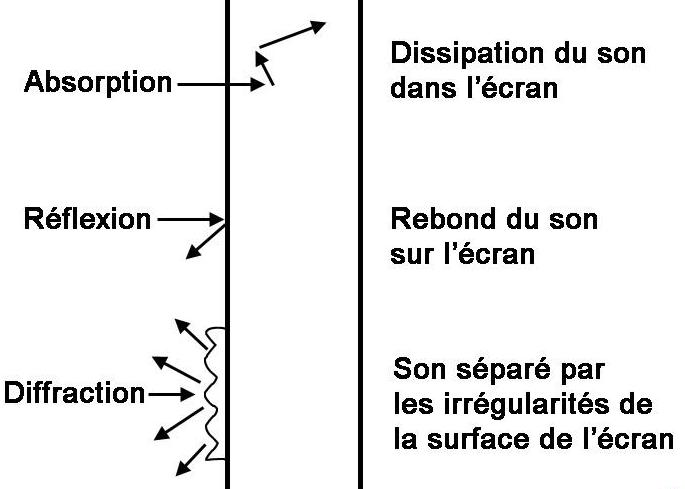
\includegraphics[width=0.5\linewidth]{images/schema_ecran_antibruit}
	\caption[Les différents comportements d'une onde lorsqu'elle rencontre une paroi]{Les différents comportements d'une onde lorsqu'elle rencontre une paroi \footnotemark}
	\label{schema_absorption}
\end{figureth}
\citefnt[Chap. 1]{aquaterra}

En se plaçant en un point à l'intérieur de la salle, on pourra alors recevoir un signal sonore comme étant la somme d'un champ direct et d’un champ réverbéré. Le son direct provient directement de la source sans avoir touché aucune surface. Le son réverbéré se distingue en deux catégories : les premières réflexions dont l'ensemble forment la texture du son et le champ diffus qui peut être assimilé à une somme infinie d'ondes se propageant dans toutes les directions \cite[p. 9]{jouhaneau}.
On comprend alors que les principaux facteurs qui vont influer sur l'acoustique perçue dans une salle sont : la source sonore, le milieu de propagation et la nature des parois et des obstacles.

\begin{figureth}
	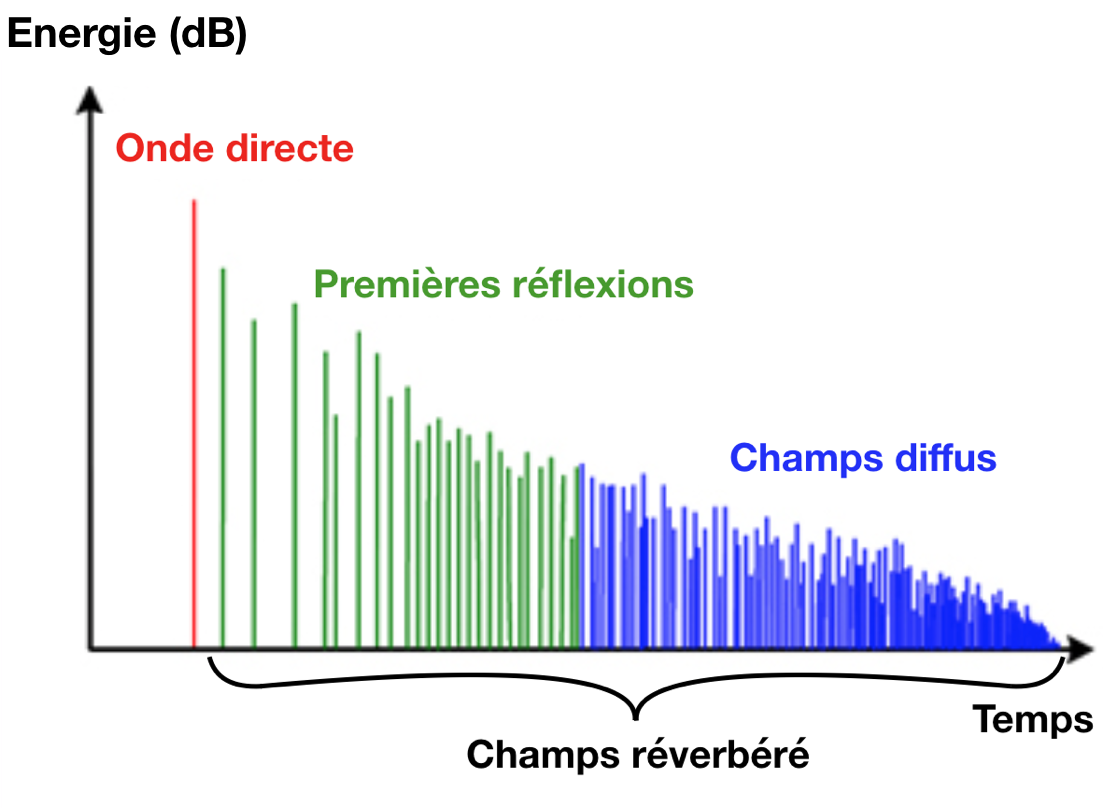
\includegraphics[width=0.7\linewidth]{images/RIR_schematique}
	\caption{Réponse temporelle d'une impulsion sonore dans une salle}
	\label{RIR_schematique}
\end{figureth}

La figure \ref{RIR_schematique}, illustrant la \gls{rir}, montre que l'information perçue est une succession d'ondes sonores arrivant décalées dans le temps. Si l'écart entre ces ondes est long, alors d'auditeur pourra les différencier et entendra le phénomène d'écho. Au contraire, si l'écart est suffisamment restreint et que les ondes sont mélangées au moment d'arriver à l'auditeur, alors celui-ci n'entendra qu'un son prolongé dont l'intensité diminue. Il s'agit de la réverbération \cite[p. 39]{sabine}. 





\subsection{Notion de flux d'intensité acoustique} \label{sect_intensite}
On définit par intensité acoustique la puissance transportée par les ondes sonores, par unité de surface, mesurée perpendiculairement à la direction de ce transfert \cite[IEC 60050]{cei}. Cette notion permet d'étudier le son perçu par les humains on la reliant à la pression acoustique qui va s'exercer de proche en proche dans l'air jusqu'à atteindre le tympan. Ainsi, la puissance sonore transportée par l'onde acoustique sera mesurable en un point de l'espace. Toute la puissance sonore mesurée en un point a une origine (actuelle ou passée) dans un flux d'énergie provenant d'une ou plusieurs directions identifiables. L'intensité acoustique mesure le flux résultant de ces transferts. 

L'intensité acoustique est un vecteur ayant pour origine le point de mesure et de même direction que le vecteur vitesse de l'onde. On peut l'écrire comme la moyenne dans le temps de l'intensité acoustique instantannée :

\begin{equation} 
\overrightarrow{I}(\overrightarrow{d},t) = \frac{1}{T} \int^T_0 p.\overrightarrow{v}dt
\end{equation}

Le flux de l'intensité acoustique instantanée à travers une surface sphérique $S(t)$ donnée correspond à l'énergie acoustique $E(t)$ transférée à travers cette surface, à l'instant considéré :

\begin{equation} 
E(t) = E_0 \int_{S(t)} \overrightarrow{I(t)}.\overrightarrow{dS} \qquad \forall t > 0
\end{equation}

L'acoustique suit le premier principe de la thermodynamique selon lequel il y a conservation d'énergie. Ainsi : 
\begin{equation} 
\int_{S(t)} \overrightarrow{I(t)}.\overrightarrow{dS} = 1 \qquad \forall t > 0
\end{equation}

Après intégration sur la surface sphérique, nous pouvons écrire l'intensité acoustique infinitésimale :
\begin{equation} 
 \overrightarrow{I(t)} = \frac{1}{4\pi  \overrightarrow{d}(t)^2} \qquad \forall t > 0
\end{equation}

\begin{figureth}
	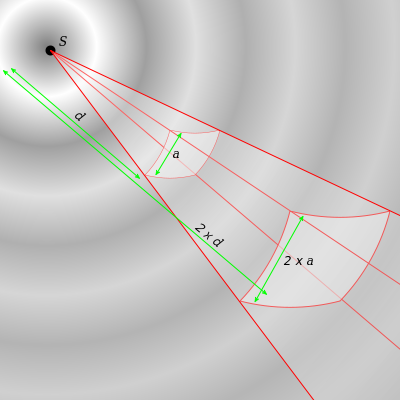
\includegraphics[width=0.5\linewidth]{images/flux}
	\caption{Représentation de la répartition du flux énergétique dans la propagation d'une onde sphérique}
	\label{flux}
\end{figureth}

On comprend que l'intensité décroit comme le carré de la distance et qu'une portion d'énergie considérée va donc être portée par un angle solide (voir fig. \ref{flux}). Sur une portion $\sigma$ l'énergie est portée par l'angle solide correspondant $\Omega_{\sigma}$ telle que :

\begin{equation} \label{eq_energie}
E_{\sigma}(t) = E_0 \int_{\sigma}  \frac{1}{4\pi  \overrightarrow{d}(t)^2} \overrightarrow{dS} = \frac{E_0}{4\pi}  \Omega_{\sigma}
\end{equation}


Par ailleurs, l'étude d'un signal sonore qui interagit avec un milieu ou un obstacle tel qu'un tympan par exemple se fait en pression ($N/m^2$ ou $Pa$). En conditions de champ libre, l'énergie acoustique est proportionnelle au carré de la pression acoustique :
\begin{equation} 
E_i \propto p^2
\end{equation}



\subsection{Absorption atmostphérique}
 \label{sect_absAIr}
Pour se rapprocher d'un modèle réaliste de propagation d'onde, il est important de prendre en compte l'absorption atmosphérique. Ce phénomène est dû à la viscosité et la conduction thermique du milieu ainsi qu'à l'absorption des molécules. Ces effets vont provoquer une décroissance exponentielle de l'énergie d'onde \cite[p. 68-70]{jouhaneau}. Selon leur distance parcourue dans l'air, l'intensité acoustique va subir une atténuation en prenant en compte trois facteurs principaux : la température, l'humidité et le pression. La température et la pression atmosphérique de référence sont respectivement de 20°C et 101,325 kPa \footnote{International Standard Atmosphere}. Le coefficient d'atténuation dépend de la fréquence du son et peut être obtenue d'après les formules analytiques de la norme ISO-9613-1. 

% view-source:http://resource.npl.co.uk/acoustics/techguides/absorption/
Tout d'abord, nous calculons le facteur d'humidité $h$ correspondant à la concentration molaire de vapeur d'eau \cite[Annexe B, B.1]{iso} :

\begin{align}
	C_h & = 4,6151 - 6,8346 \times \frac{273,15}{T}^{1,261} \\
	h & = hum \times 10^{\frac{C_h}{P_r}} \\ 
\end{align}

Avec : \\
$T$ : La température en Kelvin \\
$P_r$ : La pression relative ($P_r = \frac{P_{abs}}{101,325}$) \\
$hum$ : L'humidité relative \\

Nous exprimons ensuite les fréquences de relaxation de l'oxygène et de l'azote \cite[6.2, eq. 3 et 4]{iso}:

\begin{align}
	fr_O & =  P_r \times (24 + \frac{40400 \times h \times (0,02 + h)}{0,391 + h})  \\
	fr_A & =  \frac{P_r}{\sqrt{T_r}} \times (9 + 280 \times h \times \exp^{-4,17 \times (\frac{1}{\sqrt[3]{T_r}} - 1)})
\end{align}


Avec : \\
$T_r$ : La température relative à 20°C ($\frac{T}{293,15}$) \\
$f$ : La fréquence en Hz \\

Nous pouvons alors exprimer le coefficient d'absorption de l'air en dB/m en fonction de la fréquence  \cite[6.2, eq. 5]{iso} :

\begin{equation}
	Abs = 8,686 \times f^2 \times (\frac{1,84 \times 10^{-11}}{P_r} \times \sqrt{T_r} + T_r^{\frac{-5}{2}} \times (0,01275 \times \frac{\exp{\frac{-2239,1}{T}}}{fr_O + \frac{f^2}{fr_O}} + 0,1068 \times  \frac{\exp{\frac{-3352}{T}}}{fr_A + \frac{f^2}{fr_A}}))
\end{equation}

\begin{figureth}
	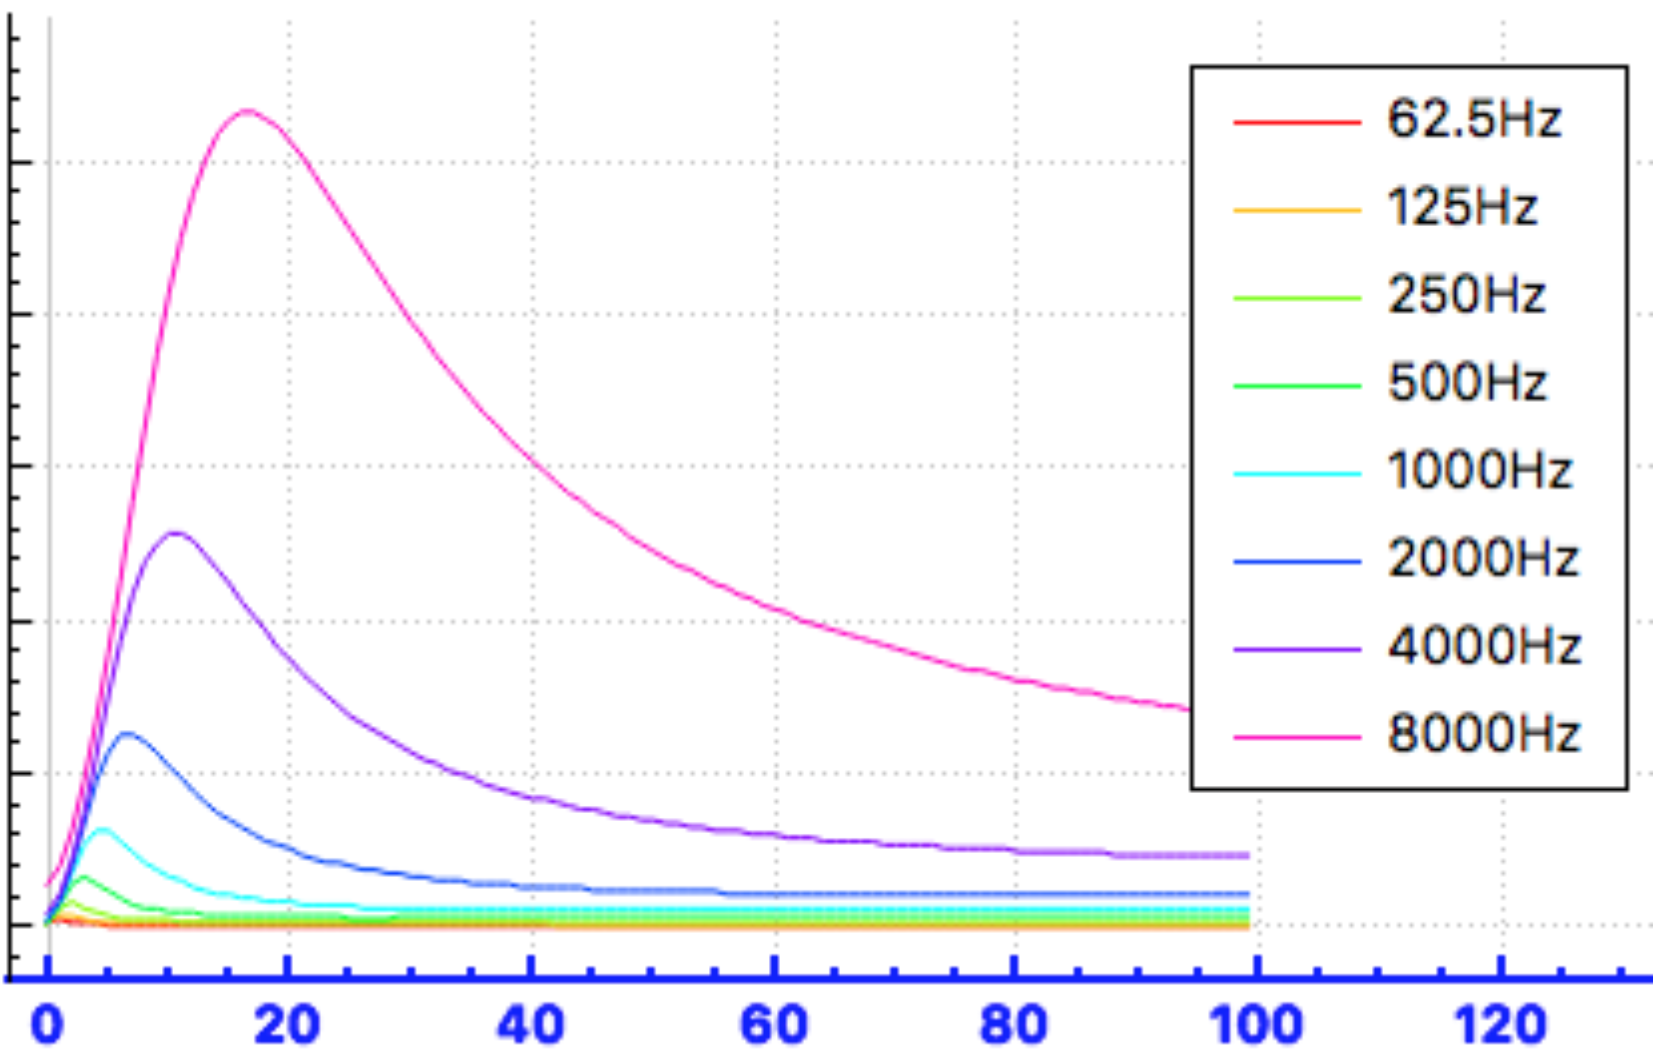
\includegraphics[width=0.8\linewidth]{images/courbesAbs}
	\caption{Courbes d'absorption de l'air en fonction de l'humidité relative (\%)}
	\label{courbesAbs}
\end{figureth}











\section{Méthodes de calcul acoustique} 
Le calcul de l'acoustique d'une salle peut se faire selon différentes méthodes. Nous allons succinctement en présenter quelques unes afin d'en dégager les grands principes et les limites.

	\subsection{Principe statistique}

P. E. Sabine écrit en 1932 "\textit{Acoustics and architecture}" en reprenant les principes son homonyme W. Sabine. Ce dernier décrivait 20 ans plus tôt des protocoles de test pour mesurer des temps de réverbérations dans les salle. P.E.Sabine considère que la réverbération suit un modèle purement statistique. De son point de vue, la densité d'échos à prendre en compte est suffisamment importante pour considérer le phénomène comme pseudo-aléatoire. \cite[p. 19]{Kandelman}. Il suppose ainsi que l’énergie sonore et le temps de réverbération sont uniformes en tout point de la salle. Il exprime la notion de libre parcours moyen en ces termes : "\textit{Pour former l’image 2D des réflexions dans une salle, on peut imaginer une boule de billard lancée au hasard sur une table et noter la variation des longueurs des trajets entre deux impacts successifs. (…) La distance moyenne de ces longueurs peut être assimilée au libre parcours moyen d’une onde sonore dans la salle}" \cite[]{sabine2}. Ces considérations permettent d'exprimer le temps de réverbération en fonction du volume de salle et l'absorption des parois comme par exemple dans la formule dite "de Sabine" : 

\begin{equation}
   	T = \frac{k.V}{A}
\end{equation}

Avec : \\
$k \approx 0,163$ \\
$V$ : le volume de la salle\\
$A$ : l'aire d'absorption équivalente telle que : 

\begin{equation}
   	A = \sum_{i=1}^N S_{i}\alpha_{i} + 4mV
\end{equation}
où : \\
$\alpha$ est le coefficient d'absorption de la i\up{e} paroi \\
$m$ est l'amortissement du milieu (par exemple l'air) \\
$S_{i}$ est la surface de la i\up{e} paroi \\
$N$ est le nombre de parois total \\

La théorie de Sabine, est encore aujourd'hui couramment employée par les acousticiens des salles. Pourtant, cette hypothèse dite de "champ diffus" n’est plus vérifiée en pratique, dès lors que la forme du milieu de propagation n’est plus homogène et que l’absorption acoustique devient importante et non uniforme. De plus, cette théorie s’applique mal aux géométries présentant des ouvertures et, en particulier, dans le théâtre d'Orange. \cite[p. 60]{picaut}. Par ailleurs, La formule de Sabine est valable tant que les $\alpha_i$ sont sensiblement inférieurs à 1. Avec le même modèle théorique, pour des valeurs de $\alpha$ plus grandes qu'environ 0,3, la formule de Eyring fournit de meilleurs résultats \cite[p. 217-241]{eyring}. Celle-ci, précisée dans les années 1920 et utilisée lors la conception acoustique de bâtiments durant leur phase de construction, est valable pour n'importe quel $\alpha$ :

\begin{equation}
   	T = \frac{k.V}{4m.V - S\ln{(1-\alpha)}}
\end{equation}

On constate que pour les faibles valeurs de $\alpha$, $\ln{1-\alpha} \simeq \alpha$ et on retrouve la formule de Sabine.
 
	\subsection{Méthode de résolution exacte} \label{sect_resExacte}

La méthode de calcul exacte d'un champs sonore consiste à résoudre une équation aux dérivées partielles avec comme conditions aux limites, les parois de la pièce. Il s'agit ainsi de mailler le domaine d'étude par des petits éléments linéiques (\gls{bem}) ou surfaciques (\gls{fem}). Sur chacun de ces éléments, on pourra calculer la pression acoustique $p(x,y,z,t)$ par résolution de l'équation d'onde de D'Alembert :
\begin{equation} 
\Delta p-\frac{1}{c^2}\frac{\partial^2p}{\partial t^2} = 0
\footnotemark
\label{alembert}
\end{equation}
\citefnt[p. 10]{Kandelman}

Avec : \\
$\Delta$ : l'opérateur laplacien\\
$c$ : la célérité de l'onde\\

Pour cela, il faudra se placer dans les conditions de l'acoustique linéaire tels que \cite[p. 19]{jot}:

\begin{itemize}
\item l'air est un fluide parfait
\item la température et la pression restent constantes
\item la vitesse macroscopique du fluide est faible devant la célérité du son
\item les fluctuations dues aux déplacements d'air sont faibles devant ces valeurs moyennes
\end{itemize}



On pourra ensuite définir les impédances complexes des parois de la salle comme conditions aux limites (\gls{Dirichlet}, \gls{Neumann}, ...). \\

Les solutions de cette équation sont les $p_i$ tels que :
\begin{equation}
p_i(x_i,t) = f_+(t-\frac{x_i}{c}) + f_-(t-\frac{x_i}{c})
\footnotemark
\end{equation}
\citefnt[p. 214-249]{alembert}

Avec : \\
$x_i$ : chacune des coordonnées de l'espace\\
$ f_+$ et  $f_-$ : des fonctions ne dépendant que d'une variable et définies à partir des conditions initiales. Elles représentent respectivement une onde se propageant sans se déformer vers $+\infty$ et $-\infty$.\\

L'équation d'Helmholtz apparait lorsque l'on cherche des solutions "stationnaires" de l'équation \ref{alembert} de D'Alembert :
\begin{equation} \label{helmoltz}
(\Delta + k^2)p(M) = f(M),	 	\qquad  \forall M  \in \Omega
\footnotemark
\end{equation}
\citefnt[eq. 2.1]{fem-bem}

Avec : \\
$f(M)$ : la distribution des sources, \\
$k$ : le nombre d'onde, \\
$\Omega  \subset R^n$ : le domaine d'étude\\

La fonction de Green est une solution élémentaire pour la source $S$ de l'équation \ref{helmoltz} de Helmoltz qui s'écrit :
\begin{equation} \label{green}
(\Delta + k^2)G(S,M) = \delta_s(M),	 	\qquad  \forall M  \in \Omega
\footnotemark
\end{equation}
\citefnt[eq. 2.2]{fem-bem}

Avec : \\
$\delta_s$ : la mesure de \gls{Dirac}, \\

\begin{figureth}
	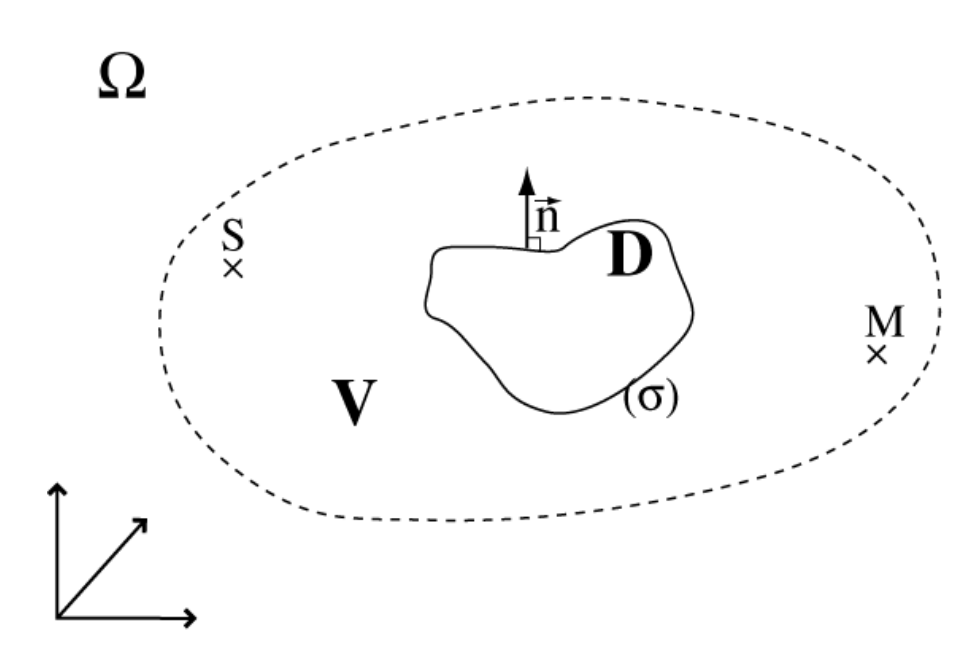
\includegraphics[width=0.6\linewidth]{images/green}
	\caption[Schéma général pour l'établissement de la représentation de Green]{Schéma général pour l'établissement de la représentation de Green \footnotemark}
	%\label{green}
\end{figureth}
\citefnt[fig. 2.1]{fem-bem}

Alors en combinant les équations \ref{helmoltz} et \ref{green}, on obtient :
\begin{equation}
G(S,M)f(M)-p(M)\delta_s(M) = G(S,M)\Delta p(M)-p(M)\Delta G(S,M),	 	\qquad  \forall M  \in \Omega
\footnotemark
\end{equation}
\citefnt[eq. 2.4]{fem-bem}

En intégrant alors cette équation sur un volume V englobant le volume D et la source S, il s'ensuit :
\begin{equation}
\int_V G(S,M) f(M) dV - \int_Vp(M)\delta_s(M) dV = \int_V [G(S,M)\Delta p(M) - p(M)\Delta G(S,M)] dV,	 	\qquad  \forall M  \in \Omega
 \footnotemark
\end{equation}
\citefnt[eq. 2.5]{fem-bem}

La  première  intégrale  dans  l'expression  ci-dessus  représente  le  champ  incident  c'est-à-dire  le  champ  rayonné  si  l'ensemble  de  sources  f(M)  était  seul  en  milieu  infini.  La deuxième  intégrale  est  le  champ  de  pression  en  un  point  M  de  l'espace  pour  une  source ponctuelle  S  (ce  facteur  serait  nul  si  la  source  S  n'était  pas  située  dans  le  volume  V).  Le membre  de  droite  peut  être  transformé  en  une  intégrale  de  surface  en  appliquant  le théorème  de  Green. Lorsque  l'on  fait  tendre  le  volume  V  vers  l'infini,  en  utilisant  la condition de Sommerfeld :
\begin{equation}
   \left \{
	\begin{array}{r c l}
		\underset{r \to \infty}{\lim} G &=& O(r^{(1-n)/2} \\
		\underset{r \to \infty}{\lim} (\delta_r G - ikG) &=& O(r^{(1-n)/2} 
	\end{array}
   \right .
   \footnotemark
\end{equation}   
\citefnt[eq. 2.3]{fem-bem}

on aboutit à une intégrale sur la surface $\sigma$ du domaine D. On obtient alors :
\begin{equation}
p(M) = p_0(M) - \int_\sigma [G(S,M) \frac{\partial p}{\partial n_S}(M) - p(M) \frac{\partial G}{\partial n_S}(S,M)] dS,	 	\qquad  \forall M  \in \Omega
\footnotemark
\end{equation}
\citefnt[eq. 2.6]{fem-bem}


C'est à partir de cette équation que l'on pourra calculer la valeur de pression acoustique en tout point M de l'espace $\Omega$ non situé sur la frontière $\sigma$ du domaine D. Cette formule peut être généralisée pour donner l'équation intégrale de Helmottz-Kirchhoff :

\begin{equation}
c(M)p(M) = p_0(M) + \int_\sigma [p(M) \frac{\partial G}{\partial n_S}(S,M) - G(S,M) \frac{\partial p}{\partial n_S}(M)] dS,	 	\qquad  \forall M  \in \Omega
\footnotemark
\end{equation}
\citefnt[eq. 2.7]{fem-bem} 

Avec : \\
\begin{equation}
c(M) = 1 - \frac{1}{4\pi} \int_\sigma \frac{\partial}{\partial n} (\frac{1}{r})dS
\footnotemark
\end{equation}
\citefnt[eq. 2.8]{fem-bem} 


Avec une dépendance temporelle en $\exp{-i \omega t}$, on peut exprimer dans $\mathbb{R}^3$ la fonction de Green sous la forme :
\begin{equation}
G(S,M) = \frac{\exp{ikr(S,M)}}{2ik}
\footnotemark
\end{equation}
\citefnt[eq. 2.29]{fem-bem} 




	\subsection{Méthodes géométriques}
	
Les méthodes géométriques sont largement utilisées dans le domaine de l'acoustique de salle. Elles se basent sur le trajet que parcourt l'onde sonore entre une source et un récepteur (fig. \ref{geometrique}). L'onde, percutant les parois subit un changement de direction de propagation et de se énergie. Chaque paroi ou obstacle porte une impédance lié à la nature de son matériau qui atténuera l'énergie de l'onde différemment selon sa fréquence.

\begin{figureth}
	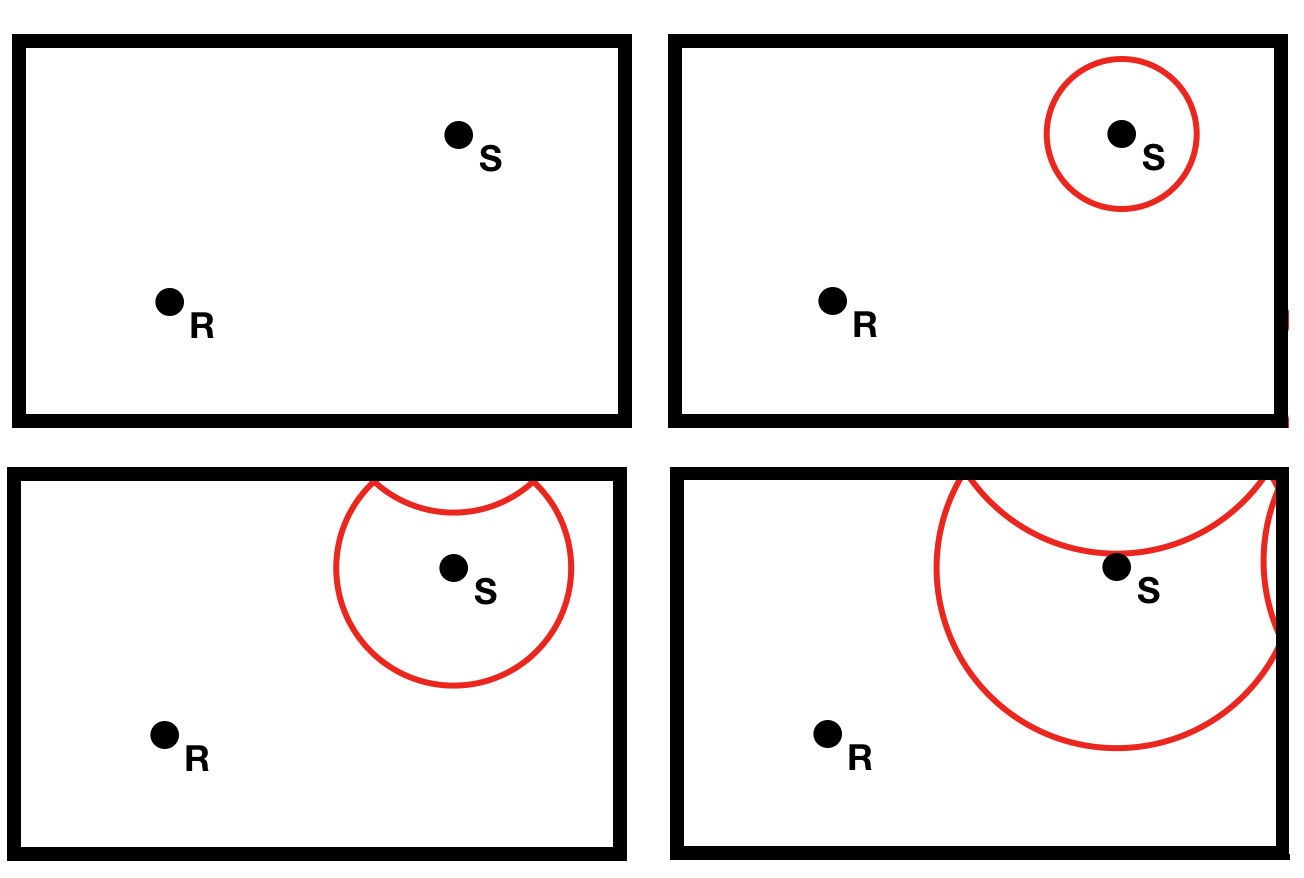
\includegraphics[width=0.8\linewidth]{images/geometrique}
	\caption{Vu 2D de la propagation d'une onde sphérique dans une salle rectangulaire}
	\label{geometrique}
\end{figureth}

En pratique certaines méthodes de calcul permet de simuler ce comportement. Tout d'abord, la méthode dite de tracé de rayon (\textit{ray-tracing}) qui est très souvent utilisée dans les logiciels d'acoustique de salle. Cette approche suppose que l’énergie sonore émise depuis une source est repartie sur un certain nombre de rayons rectilignes déviés de manière spéculaire lors de leur rencontre avec les parois. L'énergie d'un rayon sera atténuée selon le coefficient d'absorption des parois lors du rebond et décroitra comme la distance de propagation au carré afin de simuler l'effet de dispersion géométrique d'une onde sphérique. La mesure d'énergie est alors réalisée par comptage du nombre de rayons qui traversent le récepteur. La précision de mesure sera ainsi fonction du nombre de rayons émis et de la taille du récepteur. Il peut notamment y avoir beaucoup de perte d'information si le domaine de propagation est complexe \cite[p. 60]{picaut}. Il s'agit donc d'une méthode très puissante pour simuler les réflexions géométriques sur les parois mais qui devient compliquée pour simuler les effets de diffraction. Effectivement en simulant les effets de diffraction le nombre de rayons augmente considérablement à chaque réflexion et le temps de calcul devient très important. 

Pour résoudre ce problème, une approche de type "lancer de particules"sert d'alternative au tracé de rayon. Dans ce concept, chaque particule est porteuse d’une énergie constante qui ne décroit donc pas comme la distance au carré. Lors du contact avec une paroi, la particule sera réfléchie de manière statistique. Par exemple, si $\alpha$ est le coefficient d'absorption de la paroi, alors, la particule aura une probabilité de $(1-\alpha)$ d'être réfléchie et une probabilité $\alpha$ d'être absorbée. En ce sens, il est également possible de déterminer, selon une loi de probabilité, l'angle de réflexion et simuler ainsi une "pseudo-diffusion" des matériaux. \cite[p. 62]{picaut}.


Pour finir, il existe aussi la méthode dite des "sources-images" très appréciée pour son approche spatialisée des réflexions sonores. Cette méthode est fondée sur la construction de sources virtuelles, images de la source réelle, construite par symétrie par rapport aux parois de l'enceinte. La contribution énergétique de chaque source-image est celle habituellement rencontrée dans le cas de la propagation en champ libre, pondérée par le coefficient d’absorption des parois considérées \cite[p. 60]{picaut}.
Le problème de cette méthode est que l'on génère l'ensemble des sources-images d'une salle et qu'il est ensuite difficile de discriminer celles qui sont perçues et celles qui sont bloquées par des obstacles. Cela est donc plutôt adapté aux pièces de forme concave et vide. Par ailleurs, comme pour le tracé de rayons, les effets de diffraction ne sont pas pris en compte. 


\begin{figureth}
	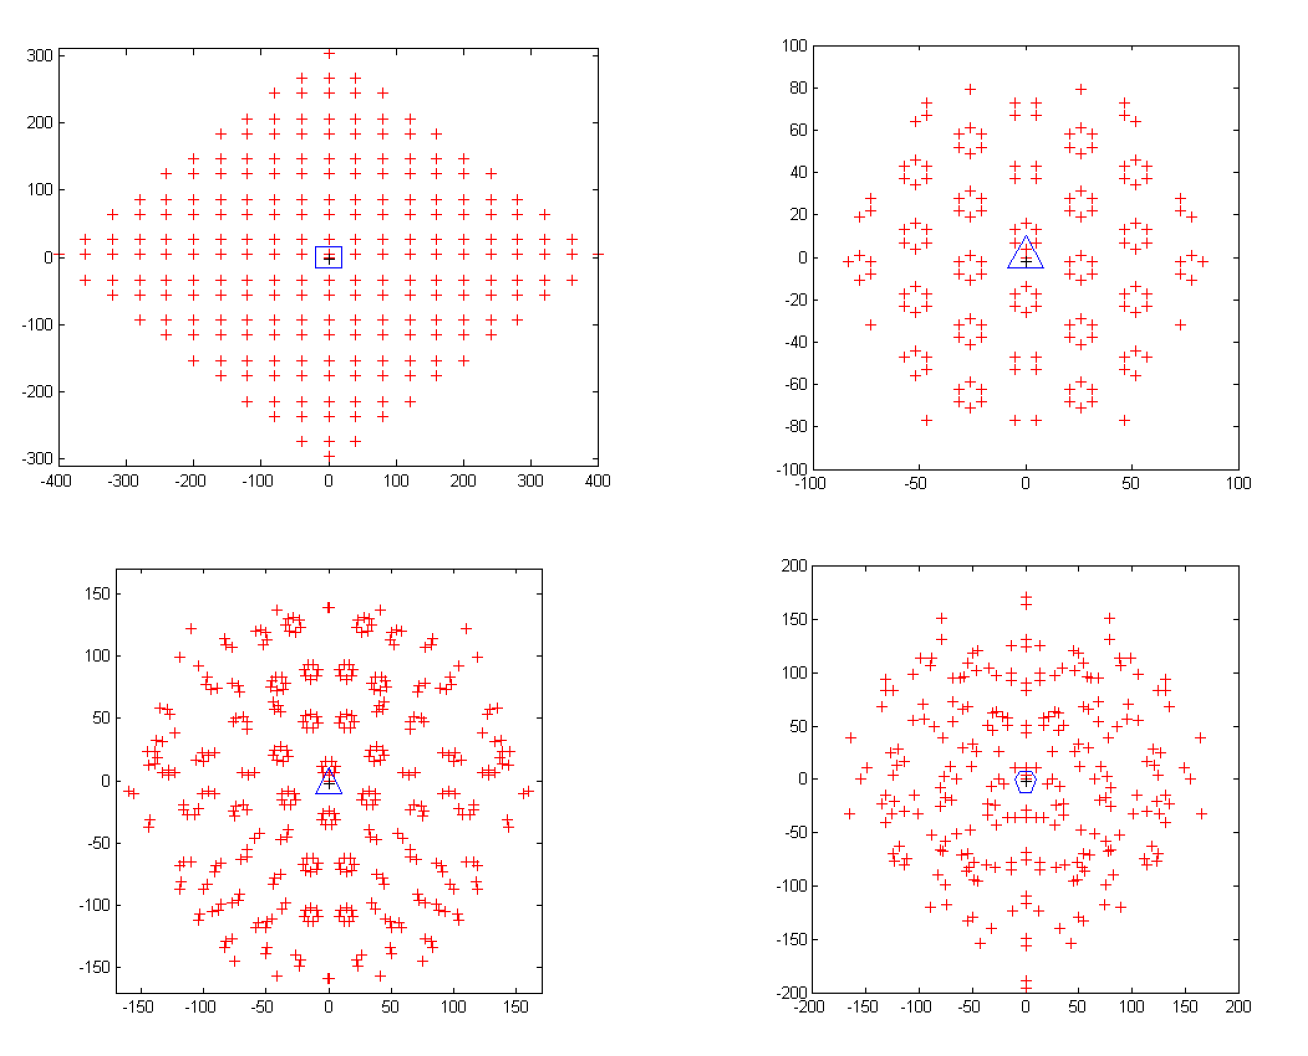
\includegraphics[width=\linewidth]{images/constellations}
	\caption[Différentes constellations de salle : la densité de sources reste constante]{Différentes constellations de salle : la densité de sources reste constante \footnotemark}
	\label{constellations}
\end{figureth}
\citefnt[Fig. 61]{Kandelman}

%C'est sur ce type d'approche géométrique que le choix s'est porté dans le cadre du projet. Nous allons donc détailler dans le prochain chapitre comment coupler ces concepts géométriques afin de répondre à la problématique. 

		
		
		
		
		
		
		
		
		
		
		
		
		
\chapter{Développement d'une méthode couplée}
	\citationChap{
	Quand on aime on ne compte pas... \\
	Ça tombe bien, je suis mauvaise en calcul !
	}{Sophie Lesellier}
	\minitoc
	\newpage
	
\section{Introduction} \label{sect_methodecouplee}
Le projet a pour essence le calcul de l'acoustique du théâtre d'Orange. Cela soulève certaines problématiques qui nous ont poussé à développer une méthode de calcul hybride. Effectivement, ce cas d'application impose le cahier des charges suivant :
\begin{itemize}
	\item Pouvoir traiter une salle de grande dimension 
	\item Pouvoir traiter un volume ouvert
	\item Prendre en compte l'absorption atmosphérique
	\item Calculer les résultats sur une large plage de fréquences audibles par l'être humain (50-8000Hz)
	\item Obtenir le son réverbéré spatialisé en tout point de l'espace
\end{itemize}

Ce dernier point permet d'étudier le déplacement de l'onde sonore. Par ailleurs, il faut pouvoir s'interfacer au modèle numérique réalisé sous Blender et décrit dans la partie \ref{part_1}. Pour cela, nous devons rajouter les caractéristiques suivantes au cahier des charges :

\begin{itemize}
	\item Utiliser un maillage surfacique sans contrainte sur la dimension ou le raffinement des faces 
	\item Pouvoir traiter plusieurs centaines de milliers de faces en un temps relativement court 
	\item Pouvoir modifier facilement les coefficient d'absorption des matériaux
\end{itemize}

Ces paramètres sont nécessaires afin de rendre l'étude acoustique du théâtre d'Orange ou de tout type de monument similaire accessible à des utilisateurs quelconques de Blender. Ainsi, la géométrie où la nature des matériaux pourra être facilement modifiable et une large série de tests comparatifs peut être mener rapidement. Le but étant de pouvoir tester des hypothèse de restitution sans avoir à multiplier les manipulations entre chaque calcul.

%Afin de répondre à ces contraintes, nous avons opté pour certains choix technologiques. Premièrement, le code est développé en C++ pour des raisons de rapidité de calcul. Il s'agit d'un exécutable "client" paramètrable directement depuis l'interface Blender. Au lancement du programme, Blender exporte le maillage dans un fichier qui sera traité par le logiciel "client". Ainsi, l'outil acoustique est transparent pour l'utilisateur et l'accès au maillage est donc immédiat. Le format de fichier s'est porté sur le \gls{obj}. Celui-ci est un des formats les plus courants et il est disponible sur la plupart des logiciels de \gls{cao}. Ainsi, l'outil n'est pas exclusif et pourra travailler à partir de n'importe quel maillage au format \gls{obj}.

Sachant cela, nous avons dans un premier temps tenté de réaliser des analyses par méthode de résolution exacte (voir section \ref{}) mais nous avons vite compris que la géométrie de la salle rendrait la résolution très difficile. Effectivement, le nombre d'éléments que doit comporter le maillage est dépendant de la longueur d'onde \cite[p. 740]{beamtracing}. Dans un cas comme le théâtre d'Orange où les longueurs se comptent en dizaines de mètres et les fréquences en kilo-Hertz (fréquences audibles), il faudra raffiner les mailles à l'échelle du millimètre, ce qui générera des milliards d'éléments. Ce genre de problème est aujourd'hui quasi-impossible à mettre en place de part la puissance de calcul et l'espace mémoire nécessaire. Par ailleurs la création d'un maillage de type conforme, c'est à dire avec des triangles de taille régulière et dont les angles ne sont pas trop aigus, représente une difficulté à part entière.
Au début du projet, nous avions tenté d'analyser une version très simplifiée du théâtre à des fréquences très faibles. Nous voulions notamment tester l'impact de la forme incurvée des gradins en comparant de manière récursive différents maillages. Le raffinement fut effectué à l'aide de l'outil "\textit{mmg}" développé à l'\gls{iscd}. Les calculs acoustiques ont été fait avec l'outil "\textit{MyBEM}" développé par le \gls{cmap}. En conservant à peu près des dimensions du théâtre, nous obtenions plusieurs centaines de milliers d'éléments et des temps de calcul déjà de quelques dizaines de minutes avec un ordinateur standard. Le constat a alors été que ce type d'étude serait trop complexe et les résultats difficiles à interpréter.

\begin{figureth}
	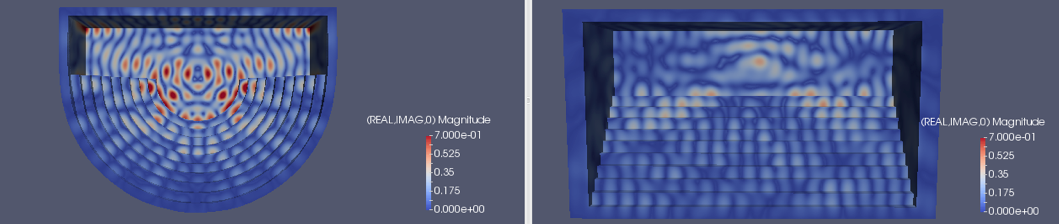
\includegraphics[width=\linewidth]{images/BEM}
	\caption{Comparaison d'un théâtre simplifié avec gradins coniques ou gradins cubiques par méthode des éléments finis de frontière à 50Hz}
	\label{BEM}
\end{figureth}

La meilleure option fut alors de se tourner vers des solutions approchées utilisant des méthodes de calcul de type géométrique. La méthode développée est dite "couplée" qui consiste à propager des rayons à partir d'une source et, à chaque réflexion sur les parois, d'analyser ceux qui traversent une sphère-récepteur. Leur temps de parcours permet de créer la \gls{rir}. Celle-ci pourra alors être convoluée à un signal audio afin de pouvoir écouter le son réverbéré (voir section \ref{sect_TDS}). Le chemin de chacun de ces rayons permet aussi de situer dans l'espace les sources-images correspondantes, c'est à dire les images de la source suite aux divers réflexions sur les parois. Nous obtenons ainsi une constellation de sources-images portant des énergies atténuées par l'absorption des parois. Cela permettra par la suite de spatialiser le son, c'est à dire de savoir d'où proviennent les différents échos. Il sera alors possible d'écouter le son réverbéré en trois dimensions. Ce chapitre vise à détailler ce processus.

\section{Notion d'onde sphérique discrétisée} \label{sect_discretise}

Comme évoqué précédemment le choix de la méthode s'oriente vers une solution géométrique dans laquelle nous allons calculer la réponse impulsionnelle à l'aide de lancés de rayons tout en créant des sources images afin de conserver l'information du parcours de l'onde dans l'espace. Dans ce développement, nous choisissons d'utiliser des sources omnidirectionelles, c'est à dire qui propagent le son de manière uniforme dans toutes les directions de l'espace. Notons tout de même qu'il serait possible d'utiliser d'autres types de sources en changeant la répartitions des rayons émis. Par ailleurs, la diffraction ne sera pas traitée même si, comme nous l'avons évoqué précédemment, il est possible d'utiliser des lois de probabilité pour répartir les rayons réfléchis selon différentes directions \cite[p.187-199]{diffusion}. Nous choisissons néanmoins de ne fonctionner qu'avec des réflexions spéculaires car le sujet de la diffraction est extrêmement vaste et complexe. Il s'agit d'un sujet à part entière que l'on ne traitera pas durant ce projet de thèse mais qui pourra venir l'enrichir par la suite.

\begin{figureth}
\begin{subfigureth}{0.55\textwidth}
	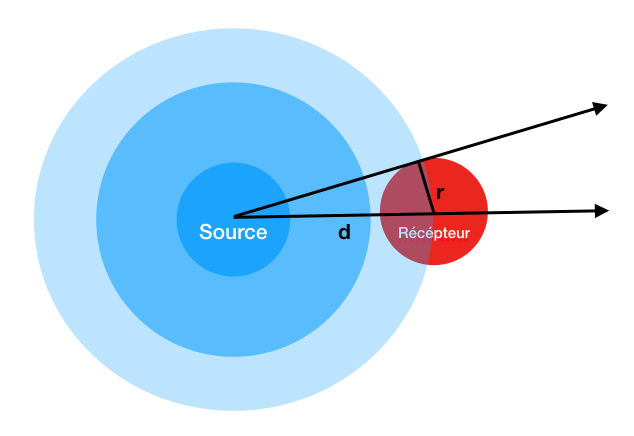
\includegraphics[width=\linewidth]{images/schema_propagation}
	\caption{Schéma en deux dimensions d'une onde sphérique dont une portion d'énergie est mesuré par un récepteur de rayon r.}
	\label{schema_propagation}
\end{subfigureth}
\qquad
\begin{subfigureth}{0.35\textwidth}
	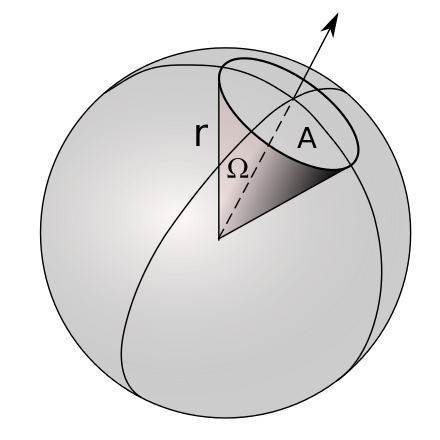
\includegraphics[width=\linewidth]{images/angle_solide}
	\caption{Représentation de l'angle solide d'un cône de révolution \footnotemark}
	\label{angle_solide}
	\end{subfigureth}
	\caption{Représentations du principe de mesure de l'angle solide}

\end{figureth}
\citefnt[image]{angle_solide}

Par ailleurs nous travaillons à partir de sources impulsionnelles. Effectivement, un signal sonore continu peut-être discretisé par une suite d'impulsions. C'est d'ailleurs le cas de tout signal numérique qui est échantillonné à une certaine fréquence. Une impulsion étant un signal d'un temps infiniment court, l'énergie émise depuis la source sera répartie sur la surface d'une sphère en expansion comme nous l'avons vu dans la section \ref{sect_intensite} (voir fig. \ref{schema_propagation}). L'énergie perçue par le récepteur sera portée par l'angle solide d'un faisceau conique (voir fig. \ref{angle_solide}). Cependant, pour simplifier les calculs, la propagation de l'onde doit être discretisée en $N$ rayons émis depuis la source de manière uniforme. Chaque rayon porte l'énergie $E_i$ tel que :

\begin{equation}
E(t) = \sum_{i=1}^N E_i(t) = \frac{E_0}{4\pi}  \sum_{i=1}^N \Omega_i
\end{equation}

Avec : \\
$\Omega_i$ : l'angle solide élémentaire tel que $ \sum_{i=1}^N \Omega_i = 4\pi$ \\



 Le problème de cette approximation est qu'elle apporte de l'erreur au résultat. Effectivement, l'information n'est plus portée par un cône mais par des rayons. Toute mesure prise entre deux rayons sera donc impossible. Il faut donc limiter au maximum cette erreur et réduire l'écart entre deux rayons. On pourra alors considérer qu'une grande quantité de rayons peut être assimilée à un cône plein. Pour cela, on souhaite connaitre la distance au bout de laquelle les rayons sont trop séparés les uns des autres pour être considérés comme un cône. On se place alors dans le cas théorique d'une source et d'un récepteur en espace libre. Il faut alors exprimer le temps au bout duquel il est possible de capter moins d'un rayon dans la sphère de mesure. 

\begin{figureth}
	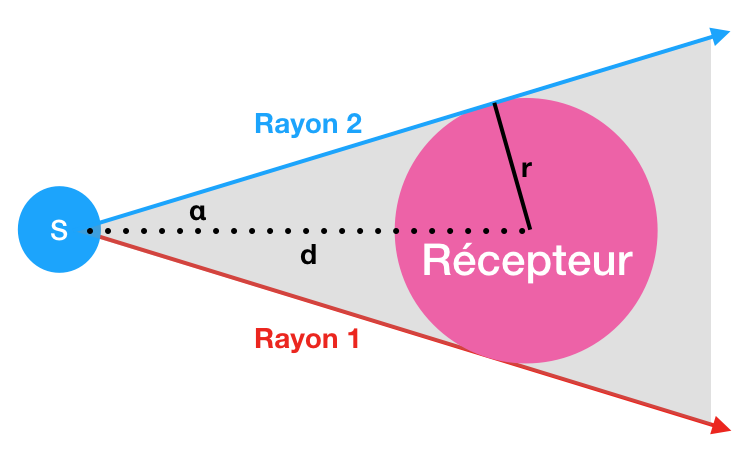
\includegraphics[width=0.8\linewidth]{images/schema_rayon}
	\caption{Schéma d'un récepteur captant au moins un rayon.}
	\label{schema_rayon}
\end{figureth}

Pour cela, nous utilisons la formule de l'angle solide d'un cône de révolution de demi-angle au sommet $\alpha$ (voir fig. \ref{angle_solide}) :
\begin{equation}
	\Omega_i = 2\pi(1-cos(\alpha)) \qquad \footnotemark 
\end{equation}
\citefnt[Angle solide d'un cône de révolution]{cone}

Or, cet angle solide peut aussi s'exprimer par :
\begin{equation}
	\Omega_i = \frac{4\pi}{N}
\end{equation}


Ainsi, pour : \\
$r$ : le rayon du récepteur \\
$d$ : la distance maximale du récepteur à la source \\
$N$ : le nombre de rayons total \\

On a, d'après Pythagore (voir fig. \ref{schema_rayon}) :
\begin{align}
	cos(\alpha) & =  \frac{\sqrt{d^2-r^2}}{d}  \\
	& =  \sqrt{1-\frac{r^2}{d^2}} \\
	%& \simeq 1-\frac{1}{2}\frac{r^2}{d^2}
\end{align}

%Car on suppose que le rayon de mesure $r$ sera petit devant la distance $d$ parcourue par l'onde. 
En normalisant l'énergie ($E_{tot} = 1$), on obtient alors :

\begin{align} 
	2\pi(1-\sqrt{1-\frac{r^2}{d^2}}) &= \frac{4\pi}{N} \\	
	\sqrt{1-\frac{r^2}{d^2}} &= 1-\frac{2}{N} \\
	1-\frac{r^2}{d^2} &= 1-\frac{2}{N} \\
	\frac{r^2}{d^2} &= \frac{4}{N^2}(N-1) \\
	 \frac{r}{d} &=  \frac{2}{N} \sqrt{N-1} \label{seuil_arret}
\end{align}


Nous constatons alors qu'en fixant $N$, le nombre de rayons d'énergie total émis depuis la source et $r$, le rayon de la sphère de mesure, nous pourrons connaitre la distance $d$ au bout de laquelle la probabilité de ne capter aucun rayon ne sera plus nulle. En pratique, on voudra réduire encore l'erreur et il faudra arrêter la mesure avant d'arriver à cet extreme. On pourra alors fixer un nombre $n$ de rayons minimum à capter. Par exemple si on fixe $n$ à 100 rayons, on s'assure que la mesure comprend au moins 100 portions de la sphère énergie et on revient statistiquement à un modèle quasi-continu.

Pour établir la nouvelle expression, il suffit de refaire les mêmes calculs en considérant que :
\begin{align}
	\Omega_i &= n.\frac{4\pi}{N} \\
	&= \frac{n}{N}
\end{align}

L'équation \ref{seuil_arret} s'écrit donc :
\begin{align} 
	\frac{r}{d} =  \frac{2n}{N} \sqrt{\frac{N}{n}-1} % \\
 	\quad \Rightarrow  \quad %\\
	 d_{max} =  \frac{N.r}{2n\sqrt{\frac{N}{n}-1}} 
\end{align}

Aussi, si $N >> n$ l'expression se simplifie par : 
\begin{align} \label{eq_dmax}
	 d_{max} \approx  \frac{r}{2} \sqrt{\frac{N}{n}}
\end{align}

Nous limitons de cette façon le calcul des premières réflexions de la réponse impulsionnelle. Cependant, les \gls{rir} sont en général calculées jusqu'à ce que l'énergie diminue de $60dB$. Il s'agit d'un critère d'arrêt classique de car il assure de couvrir la plage d'audition humaine. Or avec notre méthode, nous ne prenons plus de mesure à partir d'un certain temps, correspondant à la distance $d$. Il faudra alors jouer sur les paramètres $N$, $r$ ou $n$ pour s'assurer de dépasser le \gls{RT60}. En pratique, le temps de calcul sera très sensible à la valeur de $N$ tandis que la précision dépendra $r$ et $n$. Ainsi une possibilité est d'arrêter la mesure avant d'atteindre cette distance maximum. Il faudra alors compléter le champs diffus de manière statistique d'après les hypothèses de Sabine. La réponse impulsionnelle obtenue par tracé de rayons sera prolongée par régression linéaire pour atteindre \gls{RT60}. \\




%\begin{figureth}
%	\begin{subfigureth}{0.45\textwidth}
%		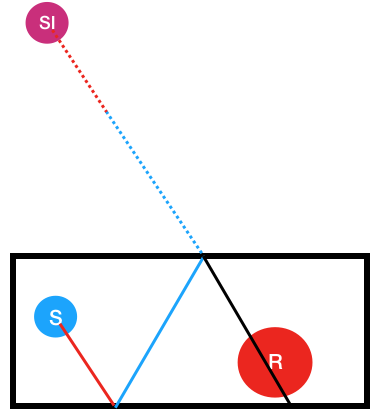
\includegraphics[width=0.9\linewidth]{images/schema_SI}
%		\caption{Schéma de la création d'une source image par réflexions successives d'un rayon sur les parois d'une salle}
%		\label{schema_SI}
%	\end{subfigureth}
%	\qquad
%	\begin{subfigureth}{0.45\textwidth}
%		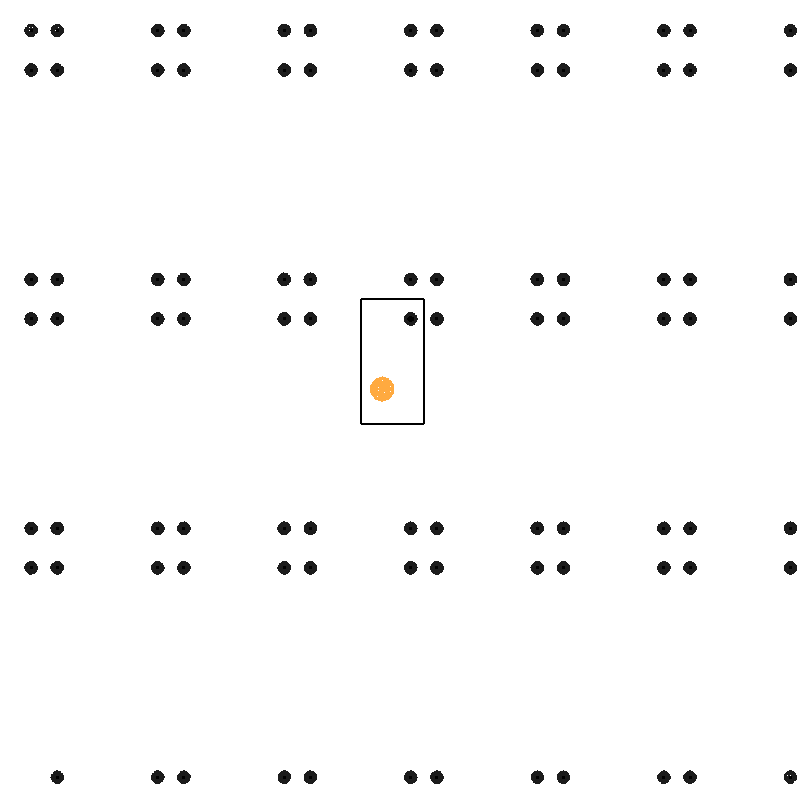
\includegraphics[width=\linewidth]{images/constellation}
%		\caption{Constellation de sources-images dans une salle rectangulaire}
%		\label{constellation}
%	\end{subfigureth}
%	\caption{Représentations du principe de sources-images}
%\end{figureth}










\section{Environnement géométrique}

\subsection{Maillage de salle et matériaux} \label{sect_lectMat}
%L'une des premières étape consiste à lire une base de données (issue du logiciel Odéon) pour récupérer les coefficients d'absorption des différents matériaux disponibles. Chaque matériau possède un numéro-référence qui devra être stipulé dans le nom du matériau sous Blender. Ces numéros sont associés dans la base de données à huit coefficients d'absorption correspondant aux bandes d'octave : 62,5Hz, 125Hz, 250Hz, 500Hz, 1kHz, 2kHz, 4kHz, 8kHz. Ces huit bandes de fréquence permettent de couvrir une large plage des fréquences audibles par l'être humain. Il existe de nombreuses bases de données recensant ces coefficients d'absorption pour tout type de matériaux. Elles sont en générales créées de manière expérimentale et celle que nous utilisons a l'avantage d'être très complète et en libre accès sur le site d'Odéon \cite[Materials]{odeon}

Comme nous l'avons vu précédemment, nous allons travailler à partir d'un maillage existant, qui sera dans notre cas d'application le théâtre d'Orange (voir partie \ref{part_1}) mais qui pourrait être n'importe quel maillage de salle. La méthode se doit donc d'être générique. Cependant notons qu'il sera obligatoire d'avoir des faces triangulaires et que les normales devront être orientée vers l'intérieur de la salle (voir fig. \ref{normales}).

\begin{figureth}
	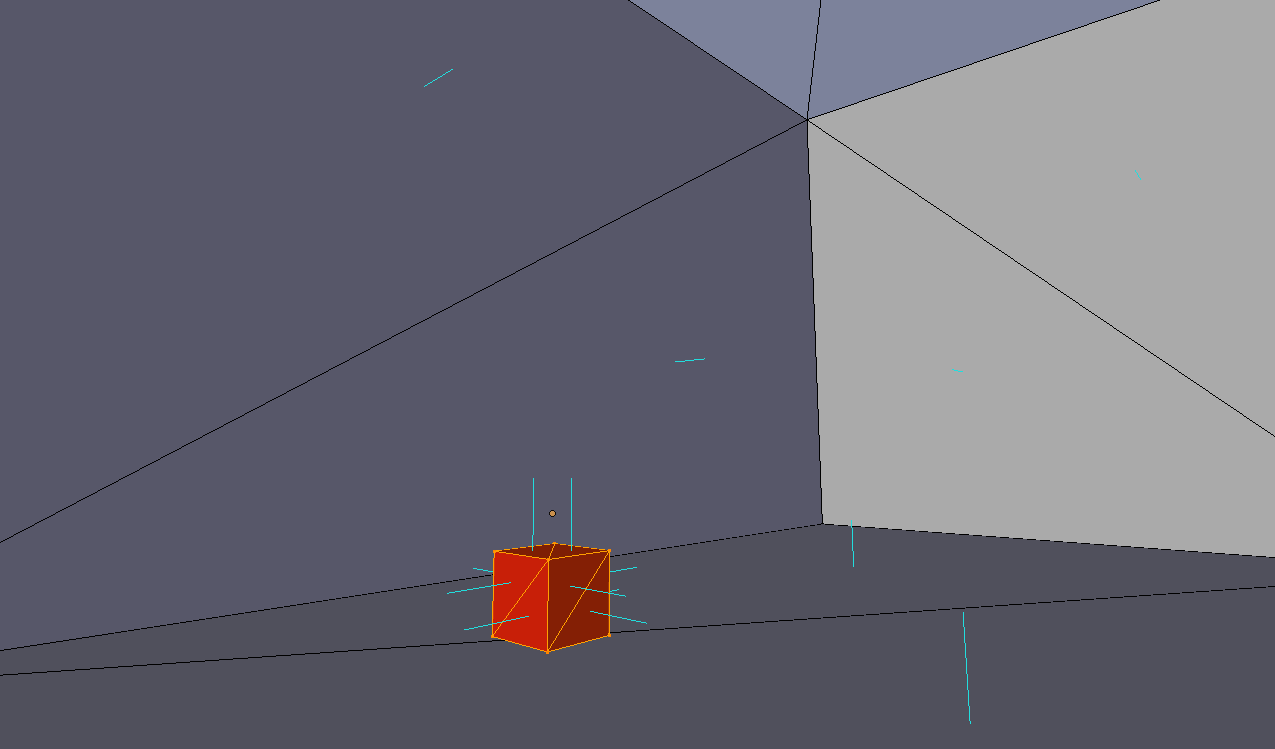
\includegraphics[width=0.8\linewidth]{images/normales}
	\caption{Représentation d'un maillages surfacique à faces triangulaires composé d'une salle et d'un obstacle et dont les normales (en bleu) sont orientées vers l'intérieur de la salle.}
	\label{normales}
\end{figureth}

Chaque face triangulaire est donc considérée comme une paroi à laquelle il faut affecter un matériau. A un matériau on associe huit coefficients d'absorption correspondant aux bandes d'octave : 62,5Hz, 125Hz, 250Hz, 500Hz, 1kHz, 2kHz, 4kHz, 8kHz. Ces huit bandes de fréquence permettent de couvrir une large plage des fréquences audibles par l'être humain. L'absorption de l'onde sonore dépendra donc de la fréquence et il faudra calculer huit réponse impulsionnelle. Il existe de nombreuses bases de données recensant ces coefficients d'absorption pour tout type de matériaux. Elles sont en générales créées de manière expérimentale et celle que nous utilisons a l'avantage d'être très complète et en libre accès sur le site d'Odéon \cite[Materials]{odeon}.\\

Voici quelques exemples de coefficients d'absorption :
\begin{tableth}
\footnotesize
	\begin{tabular}{| c | m{2.5cm} | *{8}{c|}}
		\hline
		Référence & Nom du matériau & 62,5Hz & 125Hz & 250Hz & 500Hz & 1kHz & 2kHz & 4kHz & 8kHz \\
		  \hline
		  \hline
		   1 & 100\% absorbent & 1 & 1 & 1 & 1 & 1 & 1 & 1 & 1 \\
		   \hline
		2 & 100\%reflecting & 0 & 0 & 0 & 0 & 0 & 0 & 0 & 0 \\
		   \hline
		107 & Concrete block, coarse\footnotemark & 0.36 & 0.36 & 0.44 & 0.31 & 0.29 & 0.39 & 0.25 & 0.25 \\
		   \hline
		3000 & Hollow wooden podium\footnotemark & 0.4 & 0.4 & 0.3 & 0.2 & 0.17 & 0.15 & 0.1 & 0.1 \\
	     \hline
	 \end{tabular}
	\caption{Exemples de coefficients d'absorption de la base de données Odéon}
	\label{exempleOdeon}
\end{tableth}
\addtocounter{footnote}{-1}
\footnotetext{Harris, 1991}
\addtocounter{footnote}{1}
\footnotetext{Dalenbäck, CATT}

Notons par ailleurs que l'on défini la ou les sources sonores par une position ponctuelle dans l'espace délimitée par la salle. De la même façon, le récepteur se défini par sa position dans l'espace ainsi que par son rayon de mesure. Il sera assimilé à une sphère.

\subsection{Création d'une boite englobante}

\begin{figureth}
	\begin{subfigureth}{0.55\textwidth}
		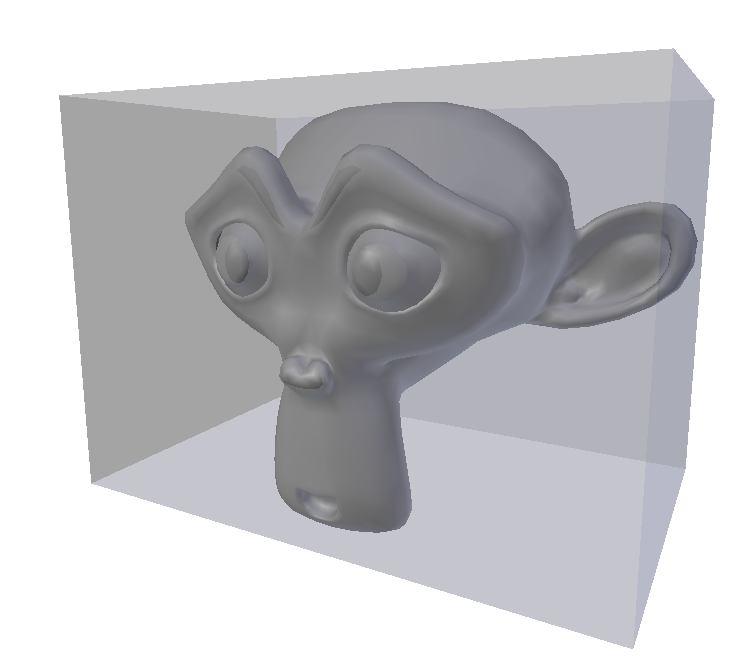
\includegraphics[width=\linewidth]{images/boiteenglobante}
		%\caption{Illustration d'une boite englobant un maillage quelconque}
		\label{boiteenglobante}
	\end{subfigureth}
	\qquad
	\begin{subfigureth}{0.35\textwidth}
		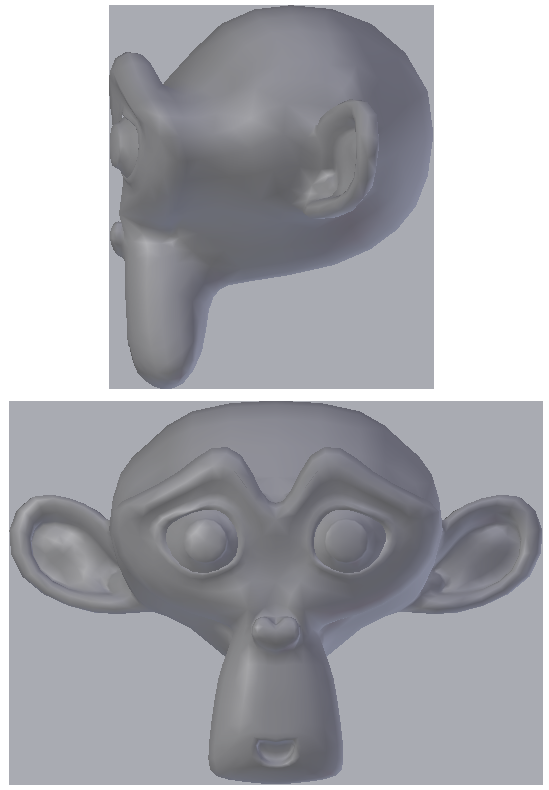
\includegraphics[width=\linewidth]{images/boiteenglobante2}
		%\caption{Illustration d'une boite englobant un maillage quelconque}
		\label{boiteenglobante2}
	\end{subfigureth}
	\caption{Illustration d'une boite englobant un maillage quelconque (Suzanne)}
\end{figureth}

La technique de lancer de rayons présente une problématique pour des maillages ouverts. Effectivement, nous verrons dans la section \ref{sect_rayon} que pour pouvoir itérer les rebonds des rayons sur les parois, il est nécessaire que tous les rayons rencontrent une face. Or, pour une salle ouverte, comme c'est le cas dans le théâtre d'Orange qui est à ciel ouvert, certains rayons peuvent ne rencontrer aucune face. Pour résoudre ce problème facilement et de manière transparente pour l'utilisateur, douze faces triangulaires sont ajoutées systèmatiquement au maillage afin de créer une boite englobante. On assigne à ces faces un matériau 100\% absorbant afin de respecter la perte d'énergie provoquée par l'absence de paroi. Par ailleurs, cette boite ne sera pas en contact avec le maillage mais sera légèrement plus grande. Ceci permet d'éviter qu'une de ces faces ne soit confondues avec une paroi réelle du maillage et que les rayons soient absorbés par la boite englobante au lieu d'être réfléchis par la paroi.




\section{Calcul des rayons} \label{sect_rayon}

\begin{figureth}
	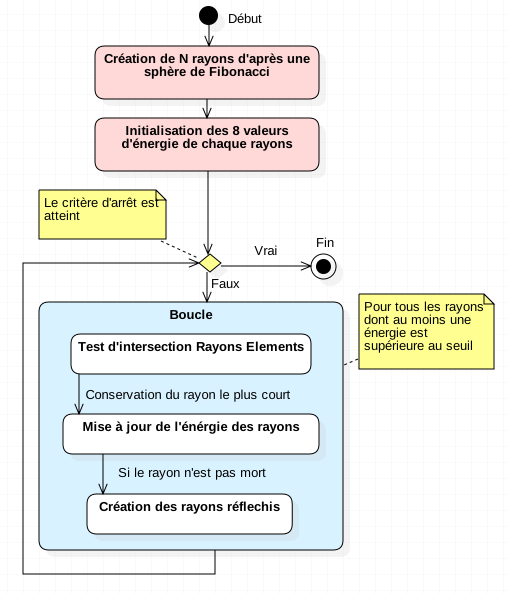
\includegraphics[width=0.7\linewidth]{images/DiagRay}
	\caption{Diagramme d'activité résumant le processus de création des rayons}
	\label{DiagRay}
\end{figureth}

Le principe de la méthode utilisée est d'émettre depuis une source des rayons se propageant en ligne droite jusqu'à atteindre un triangle du maillage. Il est bon de noter que dans la nature, les ondes sonores peuvent suivre des trajectoires courbes à cause de certains paramètres comme les gradients de température ou la présence de vent. Néanmoins nous ferons l'approximation que la propagation se fait en ligne droite. Par ailleurs, les sources sonores telles que les instruments de musique ou la voix humaine ne sont pas omnidirectionnelles mais possèdent une répartition de l'énergie qui leur est propre. Notre étude se place dans le cas général d'une source ayant une répartition uniforme de son énergie dans toutes les direction de l'espace et pourra, dans un second temps, être enrichie par d'autres types de sources. 

Pour générer une émission omnidirectionnelle de rayons, nous avons dans un premier temps évalué l'utilisation d'une "\textit{Ico Sphère}" générée par Blender. L'idée est d'utiliser le centre comme origine et chaque vertice pour calculer le vecteur directeur des rayons. Effectivement, Blender propose dans ses objets de base une sphère formée par un icosaèdre régulier. Selon le rafinement voulu, Blender découpe chaque segment en son milieu et déforme la surface pour obtenir un modèle sphérique (voir fig. \ref{icosphere}). La répartition est donc uniforme puisque l'"\textit{Ico Sphère}" n'est composée que de triangles équilatéraux identiques. Cependant, Blender bride ces subdivisions à l'ordre 8, ce qui limite l'"\textit{Ico Sphère}" à 163842 points. Outre le fait que cette manipulation aurait largement ralenti Blender, nous souhaitons pouvoir traiter un nombre de rayons bien plus important et de valeur quelconque. Nous utilisons donc une sphère de Fibonacci afin de générer les vecteurs directeurs des rayons. La formule utilisée est la suivante :

\begin{figureth}
	\begin{subfigureth}{0.45\textwidth}
		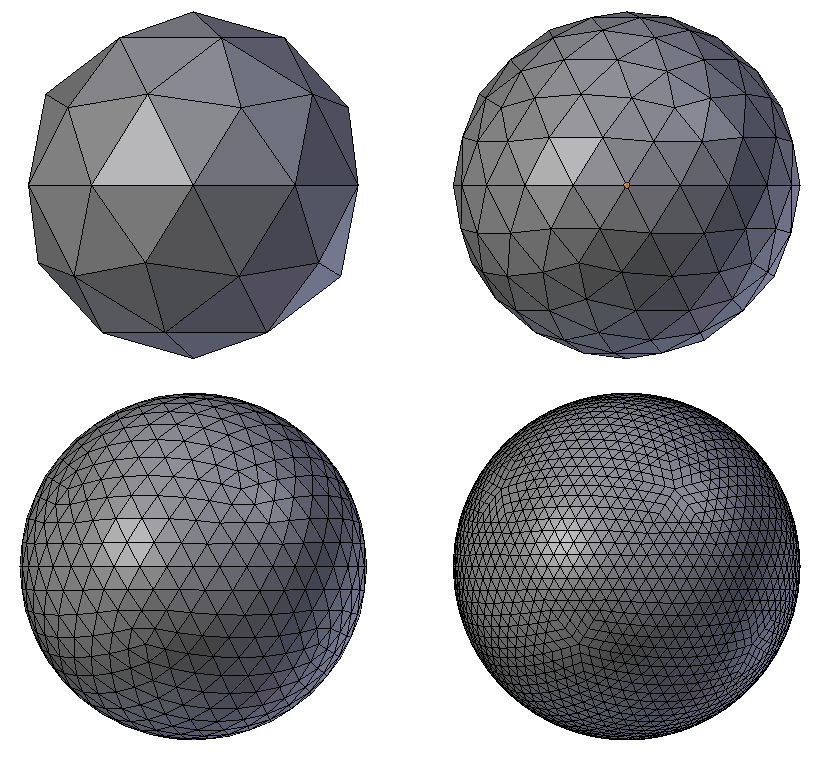
\includegraphics[width=\linewidth]{images/icosphere}
		\caption{Icosphère de Blender subdivisée 2, 3, 4 et 5 fois}
		\label{icosphere}
	\end{subfigureth}
	\qquad
	\begin{subfigureth}{0.45\textwidth}
		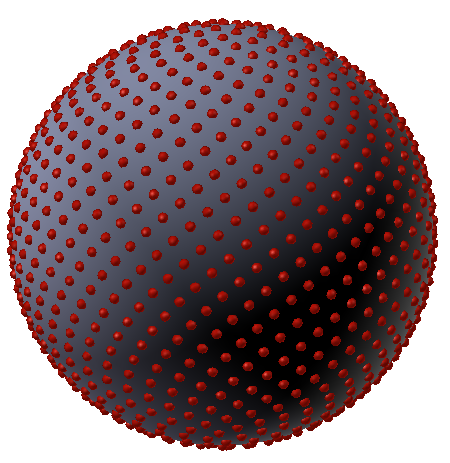
\includegraphics[width=\linewidth]{images/fibonacci}
		\caption[Sphère de Fibonacci]{Sphère de Fibonacci \footnotemark}
		\label{fibonacci}
	\end{subfigureth}
	\caption{Sphères permettant l'émission omnidirectionnelle de rayons}

\end{figureth}
\citefnt[fig. 1]{fibonacci}

\begin{align}
G_r &= \frac{1 + \sqrt{5}}{2} \\
\theta &= \frac{2 \Pi \times n}{G_r}  \pmod{2\Pi} \\
\phi &= \arcsin{(\frac{2n}{N}-1)} 
\end{align}

Avec : \\
$G_r$ : le golden ratio \\
$\theta$ et $\phi$ : les coordonnées sphériques \\
$N$ : le nombre total de rayons \\
$n \in[0, 1, 2, \ ... \ ,N-1]$ : le numéro du rayon 

A partir de ces coordonnées sphériques, on en déduit les coordonnées cartésiennes des vecteurs directeurs que l'on normalisera par la suite.
\begin{align}
x &= \cos{\phi} \times \cos{\theta} \\
y &= \cos{\phi} \times \sin{\theta} \\
z &= \sin{\phi}
\end{align}


A l'initialisation nous émettrons donc $N$ rayons depuis le centre de l'objet source et dirigés dans toutes les directions de manière uniforme. Une énergie normalisée à 1 leur est assignée. L'algorithme va ensuite fonctionner par itération jusqu'à ce que les huit énergies de tous les rayons soient toutes inférieures à une valeur seuil. Celle-ci sera typiquement de $-60dB$.  Pour cela, nous utilisons l'algorithme de Möller-Trumbore \cite[p. 2-3]{moller} développé à la fin des années 90 d'après les travaux de J.Arenberg \cite{arenberg} et D.Badouel \cite[p. 390-393]{badouel} et reconnu pour être rapide et efficace. Il s'agit d'opérer un changement de base pour le vecteur directeur du rayon et d'exprimer le point d'intersection à l'aide de coordonnées barycentriques. Cela permet d'éviter de devoir travailler avec des équations de plans et soulage les calculs.

Nous cherchons donc l'intersection entre un rayons d'équation : 
\begin{equation}
R(t) = O + Dt
\end{equation}

Et une face triangulaire de sommets $ V_0, V_1, V_2$. Un point T appartient au triangle si : 

\begin{equation} \label{eq_2moller}
T(u,v) = (1-u-v)V_0 + uV_1 + vV_2 \footnotemark
\end{equation}
\citefnt[eq. 2]{moller}

Avec :  \\
$(u,v)$ : les coordonnées barycentrique tels que $u\geqslant0, v\geqslant0$ et $(u+v)\leqslant1$. \\

Ainsi, l'intersection entre le rayon et le triangle s'écrit :
\begin{equation}
O + Dt = (1-u-v)V_0 + uV_1 + vV_2 \footnotemark
\end{equation}
\citefnt[eq. 3]{moller}

Avec : \\
$t$ : la distance entre le point d'origine du rayon et le point d'intersection. \\

D'après la règle de Cramer, nous pouvons réarranger cette équation sous la forme :


\begin{equation}
	\begin{bmatrix}
 	  -D, & V_1-V_0, & V_2-V_0
	\end{bmatrix}
	\begin{bmatrix}
 	 t \\
	 u \\
	 v
	\end{bmatrix}
	= O-V_0
	\footnotemark
\end{equation}
\citefnt[eq. 4]{moller}

Ainsi, on aura :
\begin{equation}
	\begin{bmatrix}
 	 t \\
	 u \\
	 v
	\end{bmatrix}
	=
	\frac{1}{
	\begin{vmatrix}
 	  -D, & E_1, & E_2
	\end{vmatrix}
	}
	\begin{bmatrix}
 	 	\begin{vmatrix}
 		  T, & E_1, & E_2
		\end{vmatrix} \\
 	 	\begin{vmatrix}
 		  -D, & T, & E_2
		\end{vmatrix} \\
 	 	\begin{vmatrix}
 		  -D, & E_1, & T
		\end{vmatrix}
	\end{bmatrix}	
	\footnotemark
\end{equation}
\citefnt[eq. 5]{moller}

Avec : \\
$E_1 =  V_1-V_0$ \\
$E_2 =  V_2-V_0$ \\
$T = O - V_0$ \\

Ce qui équivaut à : 

\begin{equation}
	\begin{bmatrix}
 	 t \\
	 u \\
	 v
	\end{bmatrix}
	=
	\frac{1}{
 	  (D \times E_2).E_1
	}
	\begin{bmatrix}
 		  (T \times E_1).E_2
 \\ 
 		  (D \times E_2).T
 \\
 		  (T \times E_1).D
	\end{bmatrix}	
	\footnotemark
\end{equation}
\citefnt[eq. 6]{moller}

Ainsi on pourra connaitre toutes les faces que rencontre chaque rayon et on conservera le point d'intersection pour le rayon le plus court. Effectivement, on admet que les faces peuvent absorber les rayons mais pas les transmettre donc le rayon s'arrêtera à la première face rencontrée. D'un point de vu acoustique, cela ne pose pas de réel problème à partir du moment où l'auditeur est dans la même pièce que la source. Dans ce cas, les effets de réflexions de d'absorption des parois suffisent pour retranscrire le son perçu et ce qui se passe en dehors de la pièce importe peu. Par contre si la source et l'auditeur sont séparé par une paroi, ce modèle devient faux. Dans le théâtre d'Orange, les parois sont très dense, ainsi, même si les mesures sont effectuées dans les \glspl{ambulacre} ou dans les coulisses, un modèle purement basé sur les réflexions/absorptions s'approche de la réalité. Néanmoins, certains cas ne pourront pas être testés comme par exemple la simulation de portes en bois au niveau des \glspl{parascaenium} ou bien le son entendu depuis l'\gls{hyposcaenium} situé comme son nom l'indique sous l'estrade. Il se crée alors des phénomènes de vibro-acoustique et de résonance non pris en compte. Dans notre cas, le bois ne laissera pas passer le son ce qui ne reflète pas la réalité.

Une fois que l'on sait sur quelle paroi chaque rayon va se réfléchir, on peut mettre à jour leurs énergies en les multipliant pour chaque bande de fréquence par $(1-\alpha_i)$, les $\alpha$ étant les coefficients d'absorption de la face rencontrée. La longueur totale du rayon doit être stockée afin de pouvoir prendre en compte l'absorption de l'air dans une étape ulterieur. Effectivement, étant donné que cette atténuation est assez négligeable, on ne l'affectera aux énergies d'un rayon que si celui-ci génère une source-image (voir \ref{sect_si}). Cela permet de réduire le temps de calcul global. 

Il y a alors deux possibilités pour que le processus s'arrête : 
\begin{itemize}
	\item Les énergies des huit bandes de fréquence portées par le rayon sont toutes en dessous d'un seuil. En général, ce seuil est fixé à -60dB, ce qui assure que le son ne soit plus audible.
	\item La distance totale parcourue par le rayon a dépassé un seuil déterminé par l'équation \ref{seuil_arret}. Cela assure que l'angle solide soit négligeable devant le rayon du récepteur et ainsi que la répartition discrète d'énergie puisse être considérée comme quasi-continue (voir \ref{sect_methodecouplee}).
\end{itemize}

Les rayons pour lesquels aucun de ces deux critères n'est atteint donnent alors naissance à un rayon réfléchi, les autres arrêtent de se propager. Pour calculer le vecteur directeur des rayons réfléchis, il suffit d'utiliser le vecteur normal à la face rencontrée (de norme 1) et d'utiliser la formule suivante :

\begin{equation}
\overrightarrow{r} - \overrightarrow{i} = 2 \times (-\overrightarrow{i}.\overrightarrow{n})\overrightarrow{n}
\end{equation}

\begin{figureth}
	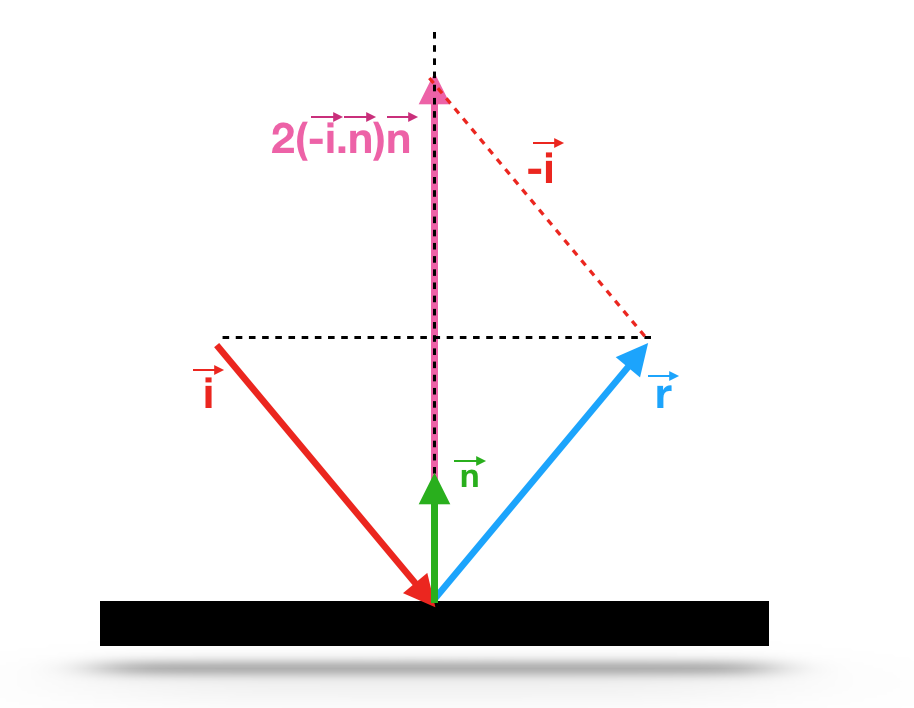
\includegraphics[width=0.6\linewidth]{images/rayRefl}
	\caption{Calcul d'un rayon réfléchi à partir d'un rayon incident et d'une normale}
	\label{rayRefl}
\end{figureth}

Nous pouvons ainsi mettre à jour les informations sur les rayons (origine et vecteur directeur) et boucler afin de propager ces rayons réfléchi svers de nouvelles faces.

Notons tout de même que dans l'implémentation algorithmique il peut se produire des problèmes d'arrondi qui peuvent faire fuir des rayons (c'est à dire qu'ils ne rencontrent aucune face). Pour éviter cela, on modifie la troisième condition de l'équation \ref{eq_2moller} en la raplaçant par $(u+v)\leqslant1.00001$. De même, si un rayon tombe dans un coin, son rayon réfléchi pourra sortir du maillage. Pour éviter cela on enlèvera systématique $1\mu m$ à la longueur des rayons.

\section{Calcul des sources-images} \label{sect_si}

\begin{figureth}
	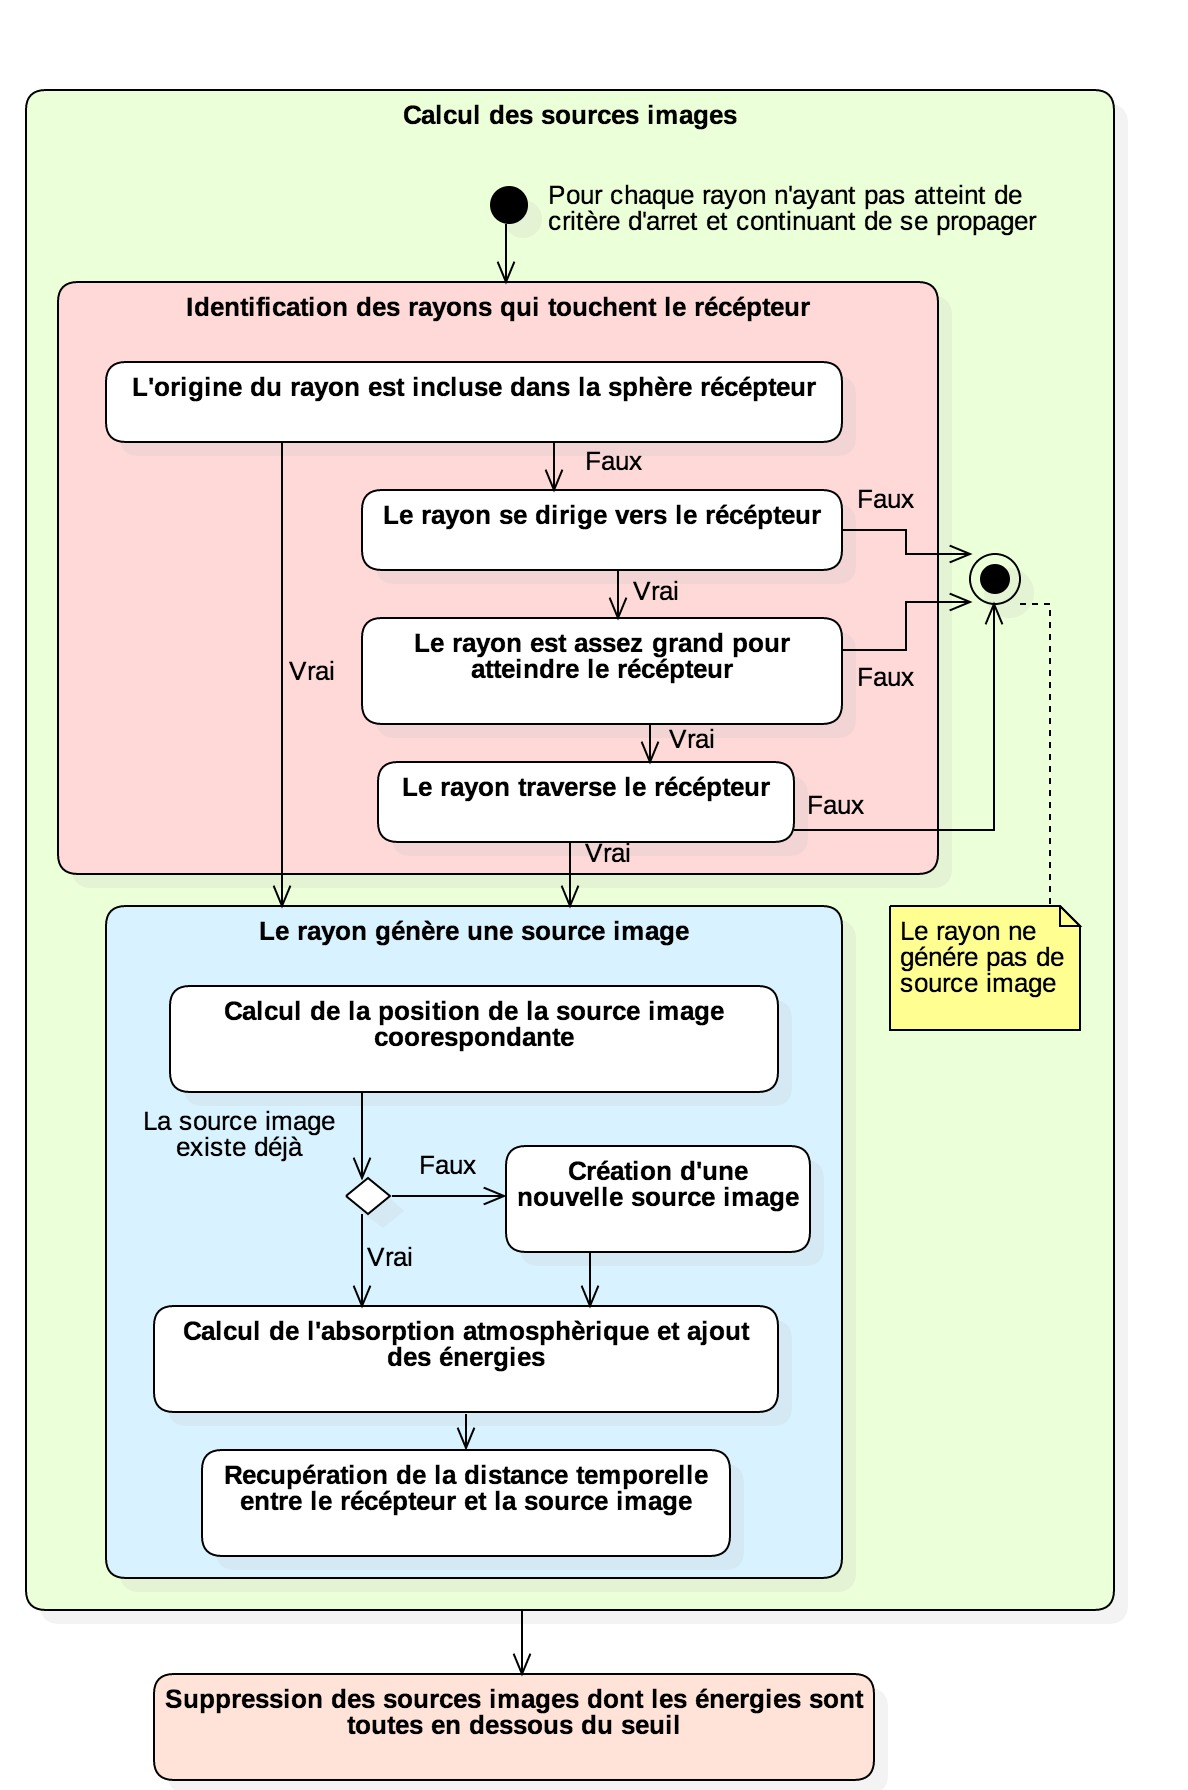
\includegraphics[width=0.7\linewidth]{images/DiagSi}
	\caption{Diagramme d'activité résumant le processus de création des sources-images}
	\label{DiagSi}
\end{figureth}

\begin{figureth}
	\begin{subfigureth}{0.55\textwidth}
			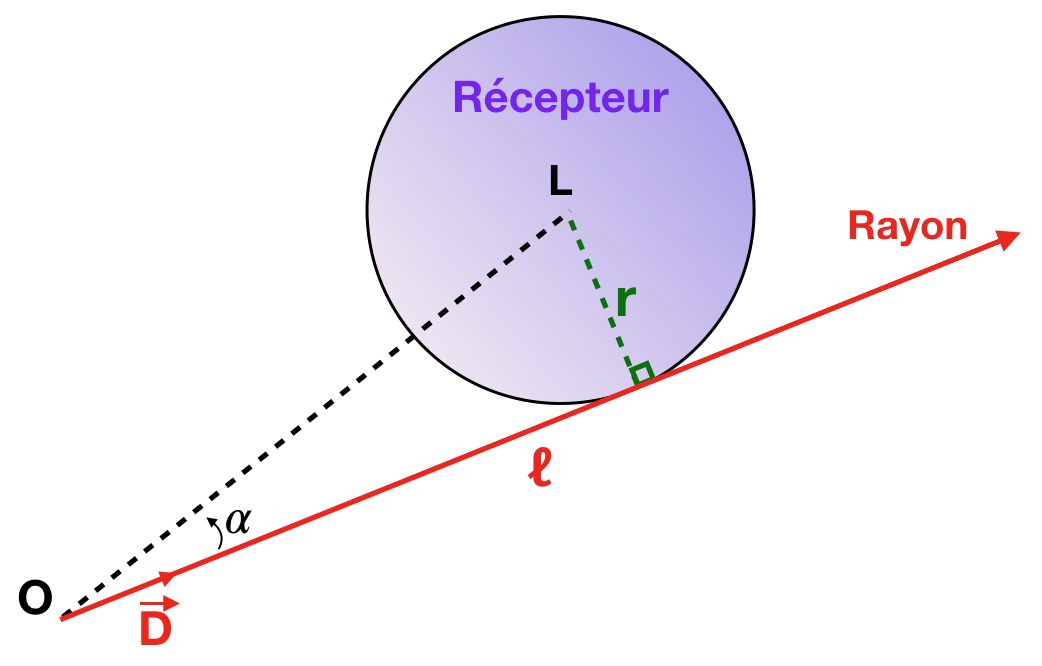
\includegraphics[width=\linewidth]{images/touche}
			\caption{Schéma d'un rayon et de la sphère récepteur}
			\label{touche}
		\end{subfigureth}
		\qquad
		\begin{subfigureth}{0.35\textwidth}
			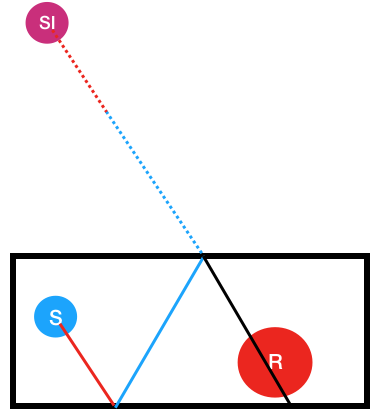
\includegraphics[width=\linewidth]{images/schema_SI}
			\caption{Schéma de la création d'une source image par réflexions successives d'un rayon sur les parois d'une salle}
			\label{schema_SI}
	\end{subfigureth}
\end{figureth}

A chaque itération, c'est à dire à chaque fois que les $N$ rayons sont entrés en contact avec une paroi et avant qu'ils ne soient réfléchis, on détermine ceux qui ont traversé le récepteur. Nous allons ainsi pouvoir ajouter au fur et à mesure des itérations de nouvelles sources-images. Pour savoir si un rayon (parmi les rayons qui n'ont pas atteints le critère d'arrêt) donnera naissance à une source image, on vérifie dans un premier temps si le point d'origine du rayon est à l'intérieur de la sphère réceptrice:

\begin{equation}
||\overrightarrow{OL}|| \leqslant r
\end{equation}

Avec : \\
$O$ : L'origine du rayon. \\
$L$ : Le centre du récepteur (Listener). \\
$r$ : Le rayon de la sphère récepteur. \\

Si c'est le cas, alors le rayon est perçu par le récepteur et une source image va être créée. Sinon, on vérifie si le rayon se dirige bien vers le récepteur. Pour cela il suffit de vérifier que :

\begin{equation}
\cos{\alpha} \geqslant 0
\end{equation}

Avec : \\
$\alpha$ : L'angle entre le rayon de vecteur directeur $\overrightarrow{D}$ et $\overrightarrow{OL}$  \\

Par ailleurs, on vérifie que le rayon est assez grand pour atteindre le récepteur (donc qu'il n'est pas interrompu par une paroi avant) :

\begin{equation}
||\overrightarrow{OL}|| \leqslant l
\end{equation}

Avec : \\
$l$ : La longueur du rayon. \\

Pour finir, on s'assure que le rayon intersecte bien la sphère récepteur :

\begin{align}
\sin{\alpha} \times ||\overrightarrow{OL}||  \leqslant r 
\quad \Rightarrow \quad
\alpha  \leqslant \arcsin{\frac{r}{||\overrightarrow{OL}||}}
\end{align}

Si ces conditions sont réunies, alors le rayon traverse bien le récepteur et une source image va être générée. Ses coordonnées seront données en traçant un vecteur de même origine mais de sens opposé au rayon courant et dont la norme sera égale à la distance totale parcourue par le rayon avant sa dernière réflexion (voir fig. \ref{schema_SI}). On assigne à cette source-image huit coefficients d'énergie correspondant aux coefficients d'énergie finaux du rayon, atténués par l'absorption de l'air sur le trajet total. Celle-ci est déterminée pour chaque bande de fréquence d'après les formules analytique décrites dans la section \ref{sect_absAIr}. Le calcul des énergies se fait de la manière suivante :

\begin{equation}
E_{si, i} = E_{r, i} \times 10^{\frac{abs_i \times l_{tot} }{10}}
\end{equation}

Avec : \\
$E_{si, i}$ : L'énergie portée par la source image sur la i-ème bande de fréquence. \\
$E_{r, i}$ : L'énergie finale portée par le rayon sur la i-ème bande de fréquence. \\
$abs_i$ : Le coefficient d'absorption de l'air sur la i-ème bande de fréquence (voir \ref{sect_absAIr}). \\
$ l_{tot}$ :La distance totale parcourue par le rayon entre la source et le récepteur. \\

Pour finir, on converti  $l_{tot}$ en temps pour pouvoir tracer le graphe temporel.

\begin{equation}
 t_{tot} =  \frac{l_{tot}}{v}
\end{equation}

Avec : \\
$ t_{tot}$ : le temps de parcours entre la source-image et le récepteur \\
$v$ : la vitesse du son dans l'air (340m/s)



\section{Génération de réponse impulsionnelle} \label{sect_rir}

Disposant de la distance temporelle entre les sources-images et le récepteur, il est possible d'afficher les courbes d'énergie sonore en fonction du temps. Aussi, pour chaque bande d'octave nous sommons les énergies par tranches temporelles. Ces tranches sont déterminées par la fréquence d'échantillonnage. Celle-ci devra être identique à celle du signal audio avec lequel la réponse impulsionnelle sera convoluée (voir \ref{sect_TDS}). Typiquement, pour une fréquence standard de 44100Hz chaque échantillons concatènera les énergies des sources-images par tranches de $22,7\mu s$. Les énergies seront ensuite normalisées pour obtenir la \gls{rir}.
 
 \begin{figureth}
	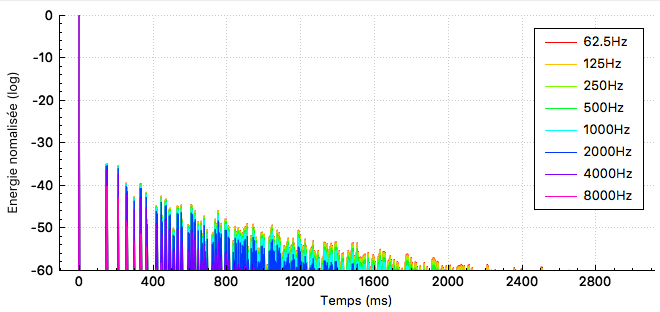
\includegraphics[width=0.9\linewidth]{images/rir}
	\caption{Exemple de \gls{rir} pour un cube de 50m d'arrête, une source et un récepteur de 20m de diamètre situés au centre, un million de rayons et une fréquence d'échantillonnage de 44100Hz}
\end{figureth}

On a vu dans les sections \ref{sect_methodecouplee} et \ref{sect_rayon} que la mesure pouvait être arrêtée avant d'atteindre le seuil limite d'audition, c'est à dire -60dB. Ce cas se présente lorsque le nombre de rayons est faible, lorsque le diamètre de la sphère récepteur est petit ou bien lorsque les rayons ont une longue distance à parcourir avant d'être suffisamment atténué (dans le cas d'une pièce fermée avec des parois très réfléchissantes par exemple). Dans ce cas, la \gls{rir} doit être complétée pour pouvoir atteindre le niveau d'énergie minimum demandé (-60dB). Pour cela, chaque courbe va être prolongée par régression linéaire afin de générer de manière statistique la queue de réverbération. D'après Sabine \cite[]{sabine} \\
A completer ...

\chapter{Optimisation algorithmique}
	\citationChap{
	Un pessimiste voit la difficulté dans chaque opportunité, un optimiste voit l'opportunité dans chaque difficulté.
	}{Winston Churchill}
	\minitoc
	\newpage
	
\section{Introduction} \label{complexite}

Afin de pouvoir qualifier les performances de l'algorithme, il est d'usage d'en mesurer la \gls{complexite}. Ce coefficient vise à analyser et qualifier le temps de calcul d'un algorithme. Dans le cas de notre méthode couplée, nous devons analyser les différentes étapes. Pour cela, on note $N$ le nombre de rayons et $M$ le nombre de faces du maillage. Premièrement, la lecture du maillage ne dépend que du nombre de faces ; la complexité de cette opération est donc linéaire de type $O(M)$. De la même manière, la création des sources-images ne dépendant que du nombre de rayons sera de complexité linéaire en $O(N)$. Celle-ci se produit en boucle tant que tous les rayons n'ont pas atteint le seuil d'arrêt. Néanmoins on ne peut pas en déterminer la  complexité car le temps de calcul dépend alors de la géométrie de la salle et des matériaux. Effectivement plus la salle est grande et plus les matériaux sont absorbant, plus vite s'arrêtera la boucle. L'étape la plus complexe est la boucle d'itération sur le calcul des rayons. Lors de cette étape, chaque rayon est testé avec chaque face. La complexité de cet algorithme est donc quadratique en $O(N \times M)$. Il s'agit de l'étape critique de la méthode et la plus chronophage.

Pour vérifier cela, nous mesurons le temps de calcul des intersections rayons-faces pour une itération (voir tableaux \ref{tabComplexite1} et \ref{tabComplexite2} et fig. \ref{complexite}). Ce test est effectué sur un MacBook de procésseur 2,7GHz Intel Core i5 avec 8Go de RAM DDR3.

 \begin{figureth}
	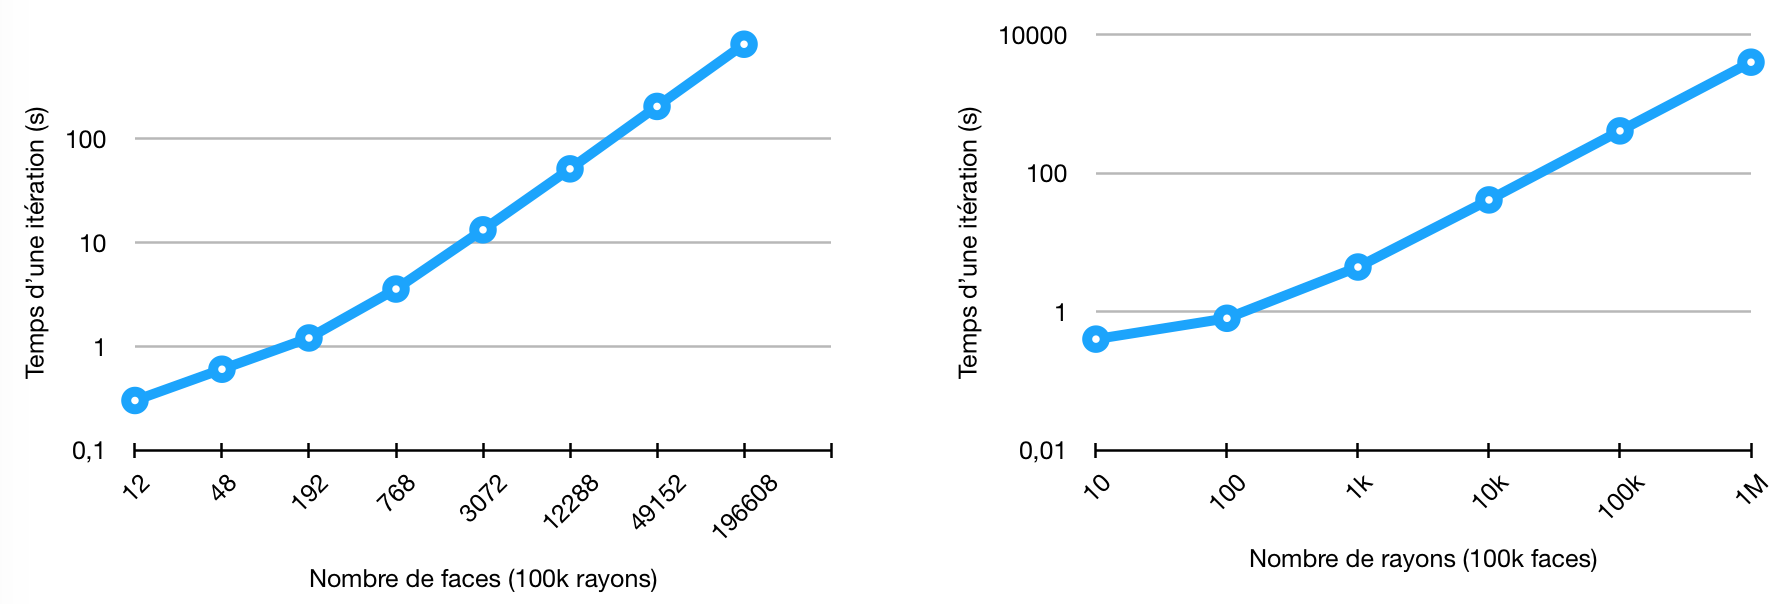
\includegraphics[width=\linewidth]{images/complexite0}
	\caption{Courbes de complexité donnant le temps (s) d'une itération en échelle logarithmique}
	\label{complexite0}
\end{figureth}

On constate comme prévue que les temps de calcul sont linéaires par rapport au nombre de faces d'une part et au nombre de rayons d'autre part ce qui donne bien une complexité quadratique. Par ailleurs, dans le cas du théâtre d'Orange, le nombre de faces est supérieur à 100 000 éléments et le nombre de rayons à émettre doit être très important compte tenu de la taille du bâtiment (voir section \ref{sect_discretise}). En testant une géométrie simplifiée du bâtiment, nous constatons que son \gls{RT60} est de l'ordre de 2 secondes. Il faudra donc pouvoir réaliser des mesures pour des rayons d'environ 700m de long. D'après l'équation \ref{eq_dmax} :

\begin{equation}
N > n(\frac{2d}{r})^2
\end{equation}

Pour une sphère de mesure de quelques mètres (celle-ci ne doit pas trop s'étendre afin que la mesure reste localisée) et $n$ de l'ordre d'une centaine de rayons, il faudra que le nombre total de rayons $N$ soit supérieur à 50 millions. En prolongeant la courbe de complexité on obtient un temps de calcul d'une trentaine d'heure, ce qui n'est pas acceptable pour entrer dans le cahier des charges. Nous devons donc optimiser l'algorithme afin de résoudre ce problème.

\section{Méthode d'octree}
\subsection{Principe général}

Comme nous l'avons vu précédemment (voir section \ref{complexite}), les maillages que nous devons traiter peuvent comporter plusieurs dizaines, voire centaines de milliers d'éléments. Les algorithmes permettant de gérer ce genre de cas utilisent souvent des méthodes de "diviser pour régner (\textit{divide and conquer})". Cela permet, notamment dans des environnements 3D de pré-trier les données afin de ne réaliser les calculs couteux en temps que sur une quantité de données restreinte. Dans notre cas, l'utilisation d'un arbre nous permettra de ne tester les interactions qu'entre certains rayons et certains éléments : ceux qui seront situés dans la même subdivision de l'espace. Sans ce tri, il serai nécessaire de tester l'intersection de chaque rayon avec chaque élément ce qui donne une complexité quadratique et ce, pour chaque itération. 

Il existe plusieurs types d'arbres permettant l'optimisation des calculs tels que les arbres binaire ou les arbres kd \\
(à compléter choix de l'arbre) ...


\begin{figureth}
	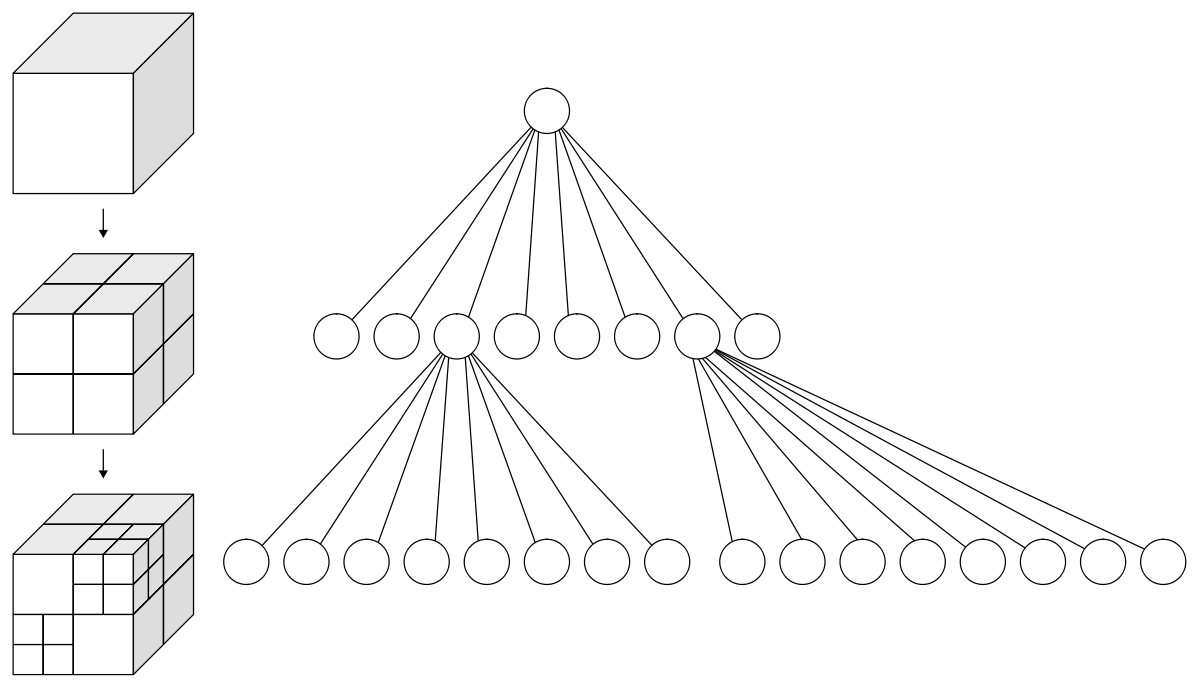
\includegraphics[width=0.6\linewidth]{images/octree}
	\caption{Illustration du principe d'\gls{octree}. Subdivision d'un cube en "octants" (gauche) et l'arbre correspondant (droite)}
	\label{octree}
\end{figureth}

Afin d'améliorer la complexité de l'algorithme décrite précedemment, le maillage va être classé dans un \gls{octree}. Cette méthode va permettre par la suite d'accélérer considérablement la vitesse de calcul \cite[p. 5]{octree} (voir section \ref{complexite}). Le principe consiste à créer une boite cubique dite "boite mère" contenant l'ensemble des éléments du maillage, c'est à dire l'ensemble des faces triangulaires. Cette "boite mère" est alors subdivisée pour créer huit "boites filles" de taille identiques qui elles-mêmes vont être subdivisées en huit "boites filles", etc (voir fig. \ref{octree}). De manière séquentielle et en descendant dans l'arborescence de l'arbre, chaque élément contenu dans une "boite mère" va être rangé dans la "boite fille" qui le contient jusqu'à atteindre une condition d'arrêt. Typiquement, l'\gls{octree} s'arrête lorsque plus aucune "boite fille" ne contient plus de $n$ éléments. Les boites seront donc raffinées de la même manière que le maillage (voir fig. \ref{octreeSuzanne}).

\begin{figureth}
	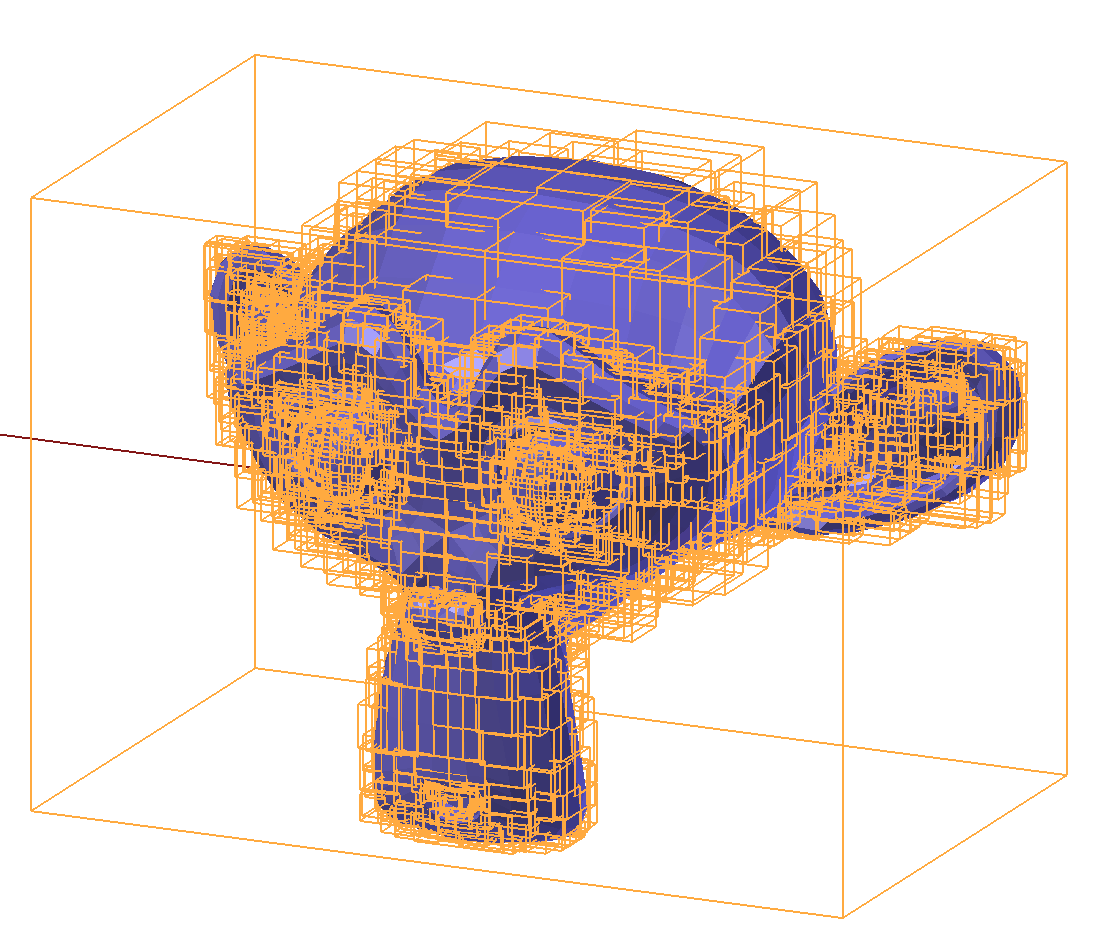
\includegraphics[width=0.6\linewidth]{images/octreeSuzanne}
	\caption{Suzanne triée dans un \gls{octree}}
	\label{octreeSuzanne}
\end{figureth}




\subsection{Implémentation}
L'algorithme a été développé de la manière suivante (voir fig \ref{DiagOctree}) :

\begin{figureth}
	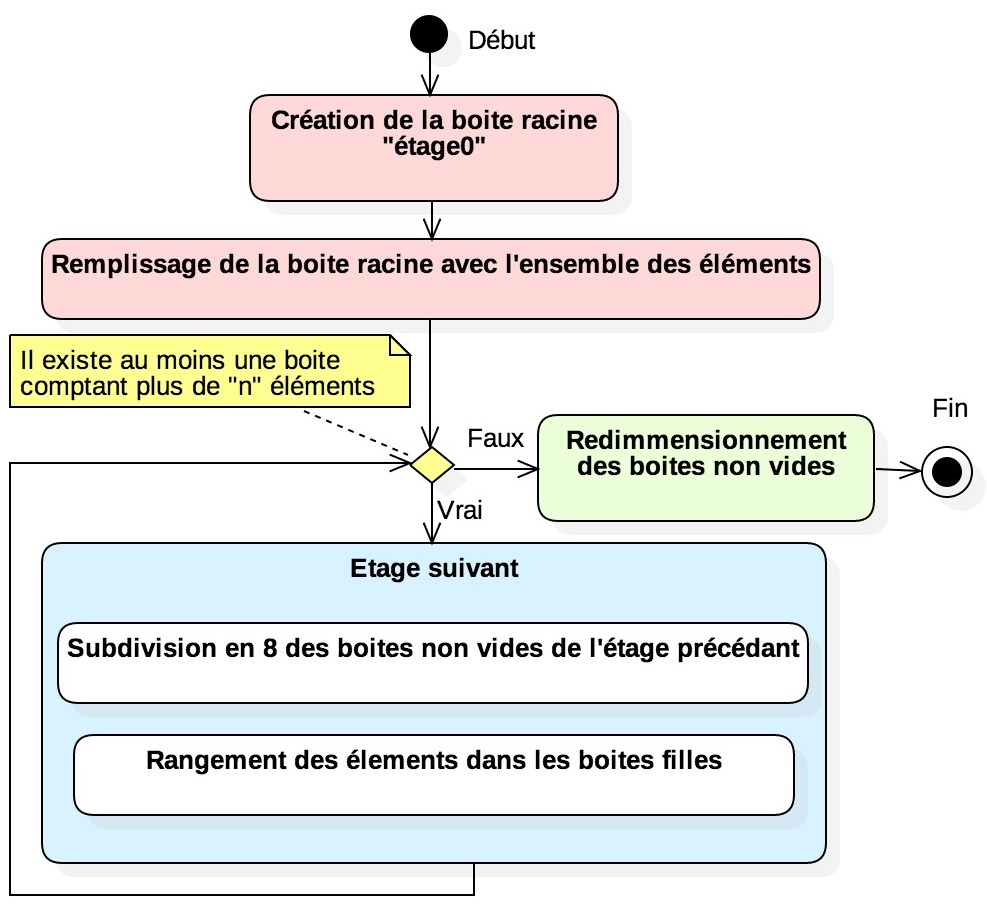
\includegraphics[width=0.7\linewidth]{images/DiagOctree}
	\caption{Diagramme d'activité résumant le processus de création d'un arbre d'octree}
	\label{DiagOctree}
\end{figureth}

Une première boite cubique englobant le maillage dans sa globalité est créée. On y associe les indices de l'ensemble des éléments puisqu'ils sont tous contenus dans cette "boite racine". On va ensuite, de manière récursive descendre dans des étages successifs. Passer de l'étage "$e$" à l'étage "$e+1$" revient à découper toutes les boites non-vides de l'étage $e$ en huit boites-filles de tailles égales qui deviendront à leur tour les boites-mères de l'étage $e+1$. Les indices des éléments assignés à une boite-mère sont répartis dans les huit "boites filles". Pour savoir quel élément appartient à quelle boite, on utilise les coordonnées du premier point de l'élément. Effectivement, un élément peut géométriquement appartenir à plusieurs boites mais il est nécessaire d'avoir unicité, c'est à dire, qu'un élément ne puisse se retrouver que dans une boite à la fois. Ainsi, chaque face triangulaire sera traitée d'après son premier point. La boucle récursive s'arrête lorsque les boites possèdent toutes moins d'éléments qu'une valeur seuil. Ainsi nous nous assurons que l'\gls{octree} se raffine de la même manière que le maillage et que chaque boite ne contient qu'un faible nombre d'éléments.


Il reste néanmoins une dernière étape qui permettra de s'assurer que les rayons rencontrent les bons éléments. Il s'agit de redimensionner les boites non-vides pour que cette fois, elles englobent bien géométriquement les faces qu'elles contiennent.



 A chaque itération sur les rayons, on va alors pouvoir classer les rayons dans l'\gls{octree} (voir nouveau diagramme d'activité des rayons, fig. \ref{DiagRay2}). Pour cela, les rayons sont assignés aux boites qu'ils intersectent à partir de la "boite racine" et en descendant dans l'arborescence de chaque branche. De la même manière que pour les triangles, les rayons sont testés avec des "boites filles" que s'ils ont bien intersecté la "boite mère" correspondante. Pour savoir si l'indice d'un rayon doit être assigné à une boite, nous utilisons un algorithme optimisé d'intersection Rayon/Boite \cite{AABB}. La particularité des boites d'un \gls{octree} est qu'elles sont toutes alignées selon les axes du repère cartésien. On appel communément ce type de boite \gls{AABB} en opposition aux \gls{OBB}. Nous allons donc utiliser cette propriété pour vérifier si un rayon intersecte une boite. Pour cela rappelons qu'un rayons peut s'écrire sous la forme : 
\begin{equation}
f(t) = D \times t + O
\end{equation}

Avec : \\
$D$ : le vecteur directeur du rayon de coordonnées $(D_x ; D_y ; D_z)$ \\
$O$ : le point d'origine du rayon de coordonnées $(O_x ; O_y ; O_z)$

On peut également exprimer les plans délimitant la boite de type \gls{AABB} par les équations suivantes :
\begin{align}
f(t) &= X_{min}  \\
f(t) &= X_{max}  \\
f(t) &= Y_{min}  \\
f(t) &= Y_{max} \\
f(t) &= Z_{min} \\
f(t) &= Z_{max}
\end{align}


\begin{figureth}
	\begin{subfigureth}{0.45\textwidth}
		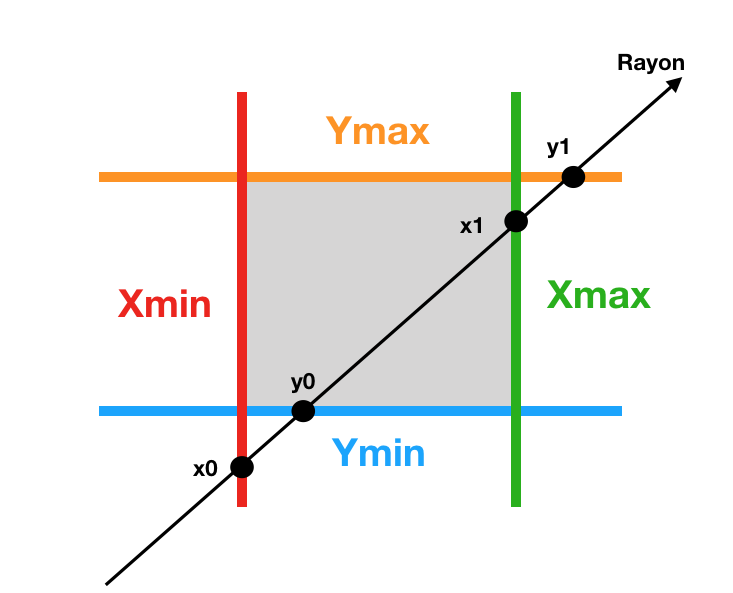
\includegraphics[width=\linewidth]{images/AABB}
		\caption{Vue 2D d'un rayon intersectant la boite}
		\label{AABB}
	\end{subfigureth}
	\qquad
	\begin{subfigureth}{0.45\textwidth}
		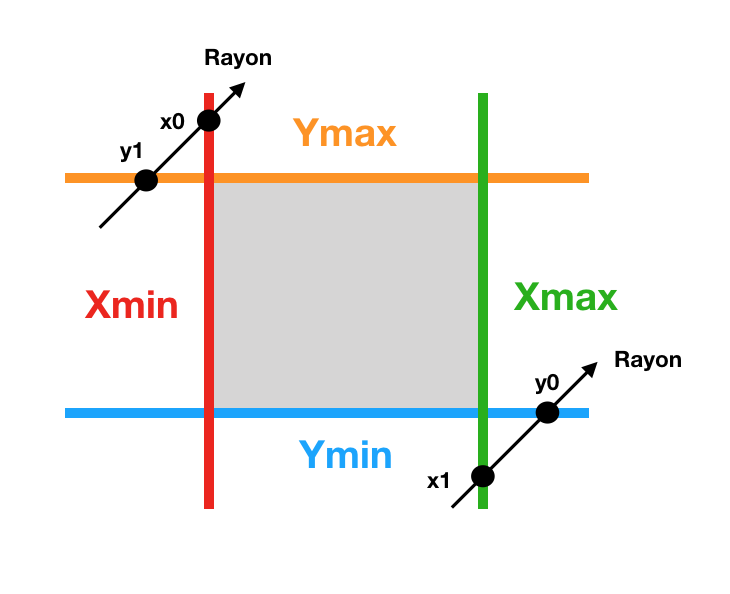
\includegraphics[width=\linewidth]{images/AABB2}
		\caption{Vue 2D de rayons n'intersectant pas la boite}
		\label{AABB2}
	\end{subfigureth}
	\caption{Illustrations de l'intersection Rayon/Boite en 2D}
\end{figureth}

Ainsi, on peut exprimer les points d'intersection entre le rayon et les plans délimitant la boite avec le système d'équations suivant :

\begin{align}
X_{min} &= x_0 \times D_x - O_x 	& \Rightarrow 	& &	 x_0 = \frac{X_{min} - O_x}{D_x} \\
X_{max} &= x_1 \times D_x - O_x 	& \Rightarrow 	& &	x_1 = \frac{X_{max} - O_x}{D_x} \\
Y_{min} &= y_0 \times D_y - O_y 	& \Rightarrow	& &	y_0 = \frac{Y_{min} - O_y}{D_y} \\
Y_{max} &= y_1 \times D_y - O_y 	& \Rightarrow	& &	y_1 = \frac{Y_{max} - O_y}{D_y} \\
Z_{min} &= z_0 \times D_z - O_z	& \Rightarrow 	& &	z_0 = \frac{Z_{min} - O_z}{D_z} \\
Z_{max} &= z_1 \times D_z - O_z 	& \Rightarrow 	& &	z_1 = \frac{Z_{max} - O_z}{D_z} 
\end{align}

On comprend d'après les figures \ref{AABB} et \ref{AABB2} que l'on va pouvoir déterminer si un rayon intersecte une boite en comparant les coordonnées des points d'intersection avec les plans. Notamment, si $x_0 > y_1$ ou $y_0 > x_1$ le rayon n'intersectera pas la boite (voir fig \ref{AABB2}). Dans le cas contraire, on appliquera le même principe sur $z$. Il n'y aura alors pas d'intersection si $max(x_0 ; y_0) > z_1$ ou $ z_0 > min(x_1 ; y_1)$. On notera que si le rayon est dirigé dans le sens inverse il faudra inverser les $\alpha_0$ et $\alpha_1$ ($\alpha$ correspondant aux coordonnées $x,y,z$) .

De cette façon les feuilles de l'\gls{octree}, c'est à dire les boites les plus basses dans l'arborescence, prendront comme arguments les indices des rayons les traversant. On pourra ainsi ne tester les intersections d'entre les rayons et les éléments situés dans les mêmes subdivisions de l'espace. Feuille par feuille, l'algorithme va donc déterminer pour chaque face les rayons qui l'intersecte et le cas échéant, sa longueur.




\section{Analyse de \gls{complexite}}

L'étape de création de l'\gls{octree} n'est pas critique car cette opération ne s'effectue qu'une seule fois au moment du chargement du maillage. Si $M$ est le nombre de faces du maillage et "e" le nombre d'étage de l'\gls{octree}, alors la complexité maximale de cette opération sera O(M.e). En pratique, comme certaines faces sont plus grande que d'autres, des feuilles vont être créées au fur et à mesure des étages et il n'y aura pas besoin de tester toutes les faces à chaque étage. La valeur de "e" dépend donc de $M$, du nombre d'éléments qu'il faut pour créer une feuille et sera fonction du raffinement du maillage. Pour une géométrie donnée, par exemple, un cube dont on augmente le raffinement [à compléter ...]

 \begin{figureth}
	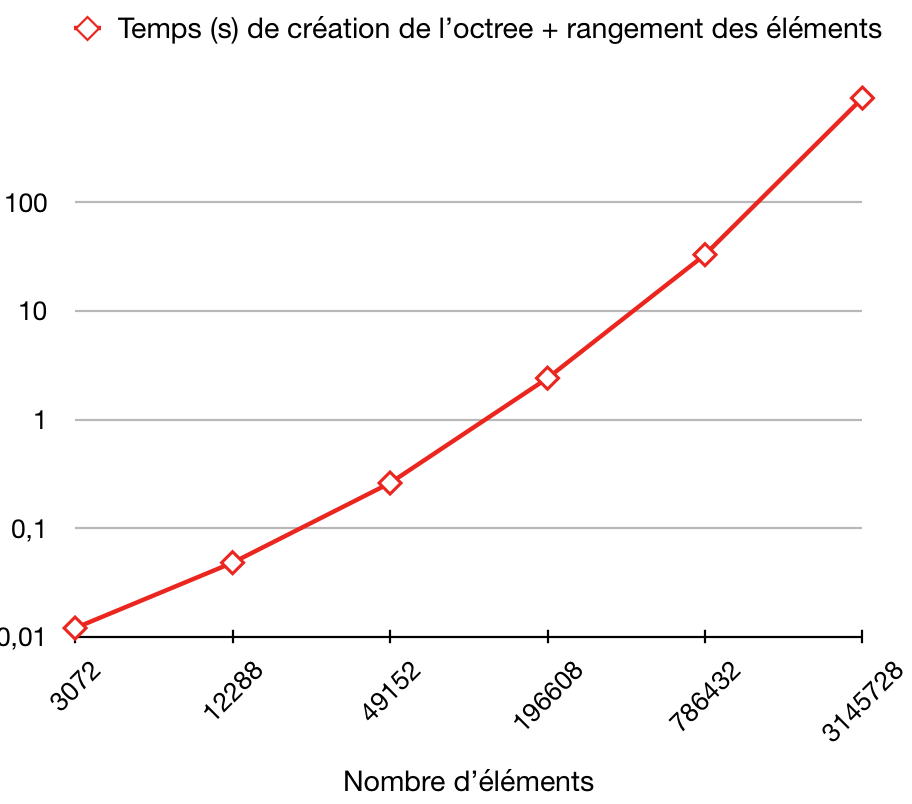
\includegraphics[width=0.4\linewidth]{images/tempsOctree}
	\caption{Temps (s) de création de l'octree sur un cube pour des feuilles comprenant 5 éléments maximum en échelle logarithmique}
	\label{tempsOctree}
\end{figureth}



Comme évoqué précédemment, l'étape critique de l'algorithme est le test d'intersection rayons/éléments car la complexité initiale est quadratique et que ce processus se répète à chaque itérations jusqu'à atteindre \gls{RT60}. Pour une itération, nous avons donc une phase de complexité linéaire

Le calcul revient finalement à assembler une matrice creuse et porte une complexité théorique de type $O(N\log{M})$. 
Pour vérifier ce comportement nous mesurons les temps de calcul d'une itération avec l'\gls{octree} et comparons avec les courbes de la figures \ref{complexite0}.


%\begin{figureth}
%	\begin{subfigureth}{0.7\textwidth}
%		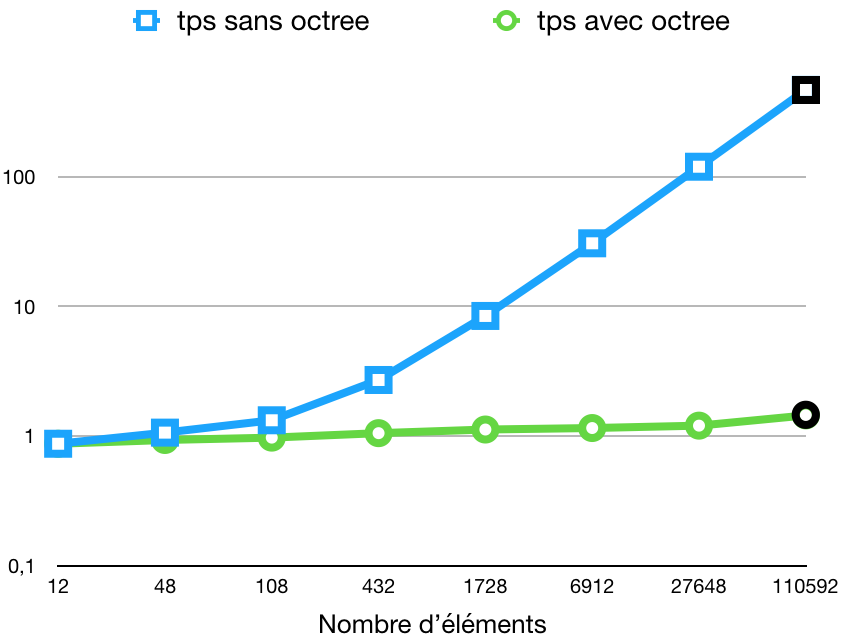
\includegraphics[width=\linewidth]{images/complexite1}
%		\caption{Temps (s) d'une itération en fonction du nombre d'éléments pour 100000 rayons (échelle log)}
%		\label{complexite1}
%	\end{subfigureth} \\
%\bigskip
%	\begin{subfigureth}{0.7\textwidth}
%		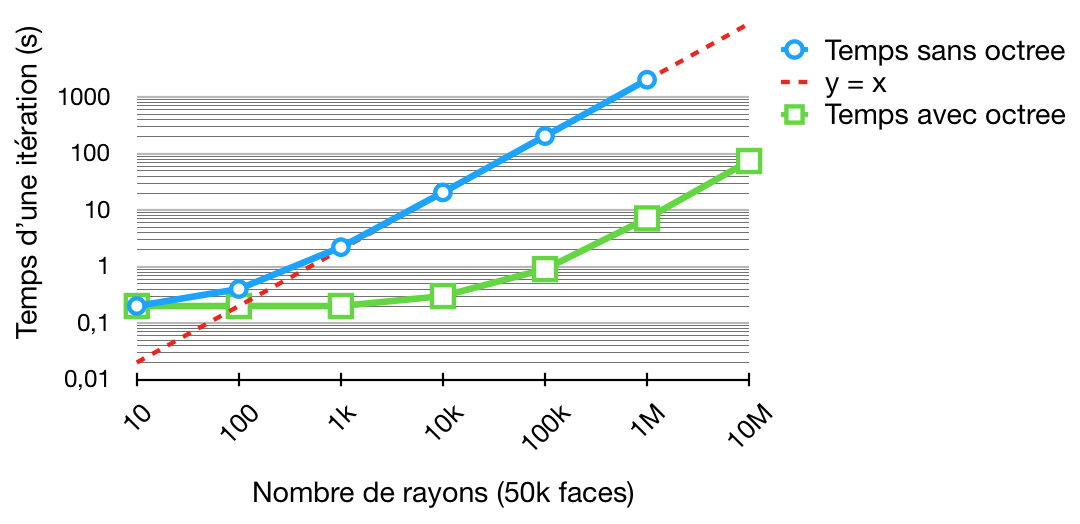
\includegraphics[width=\linewidth]{images/complexite2}
%		\caption{Temps (s) d'une itération en fonction du nombre de rayons pour 100000 éléments (échelle log)}
%		\label{complexite2}
%	\end{subfigureth}
%	\caption{Courbes de complexité}
%\end{figureth}


 \begin{figureth}
	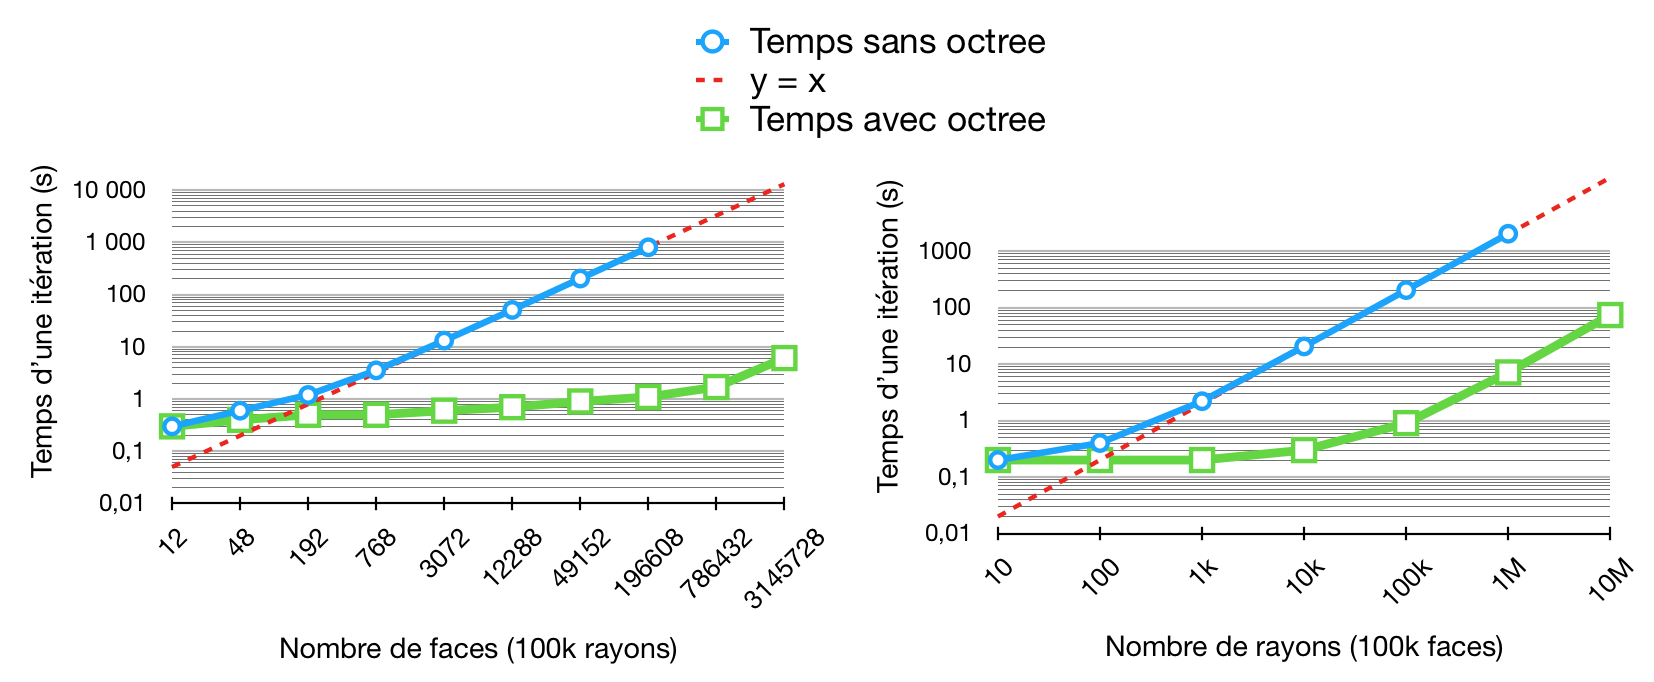
\includegraphics[width=\linewidth]{images/complexiteBis}
	\caption{Courbes de complexité donnant le temps (s) avec et sans octree d'une itération en échelle logarithmique}
	\label{complexiteBis}
\end{figureth}









\chapter{Logiciel développé}
	\citationChap{
	L'observateur modifie ce qu'il observe. Certains événements ne se produisent que parce qu'ils sont observés. Sans personne pour les voir ils n'existeraient pas. 
	}{Bernard Werber}
	\minitoc
	\newpage
	
\section{Introduction}

Dans le chapitre précédent, nous avons détaillé le fonctionnement de l'algorithme conçu pour analyser l'acoustique d'une salle. La méthode utilisée couple les principes de lancer de rayons, de sources-images et d'extrapolation stochastique. Elle vise à répondre aux problématiques de calcul acoustique en environnement complexe de manière géométrique et disrètisée. Géométrique, car seuls les effets de réflexion et absorption sont pris en compte et discrétisée car l'énergie d'onde n'est pas portée par une sphère mais par un grand nombre de rayons repartis de manière uniformes. Ainsi, il est essentiel de confirmer la justesse de ses approximations en les confrontant à des modèles théoriques. Dans ce chapitre, nous allons valider l'algorithme d'un point de vu physique et analyser ses performances. Nous présenterons ensuite son ergonomie pour l'utilisateur et et constaterons que la configuration peut se faire depuis Blender ainsi que l'analyse de certains résultats (comme l'affichage des rayons ou de la position de sources images par exemple). Nous finirons par une brève présentation du traitement du signal implémenté afin de rendre le résultat de calcul audible.


Avant de tester la justesse des résultats d'un point de vu physique, il est bon d'en vérifier la justesse géométrique. Ainsi, nous analysons si les rayons ne traversent pas les parois et que la boite englobante assure bien son rôle. Pour cela, nous importons les rayons générés par notre logiciel dans des configurations de salles simples. En propageant les rayons dans un petit labyrinthe nous confirmons qu'ils s'arrêtent bien à la paroi la plus proche et qu'ils sont ainsi contenus à l'intérieur de la salle. Nous confirmons également le bon fonctionnement de la boite englobante en utilisant une salle sans plafond ni plancher. Les rayons sont bien stoppés par une paroi invisible.

\begin{figureth}
	\begin{subfigureth}{0.45\textwidth}
		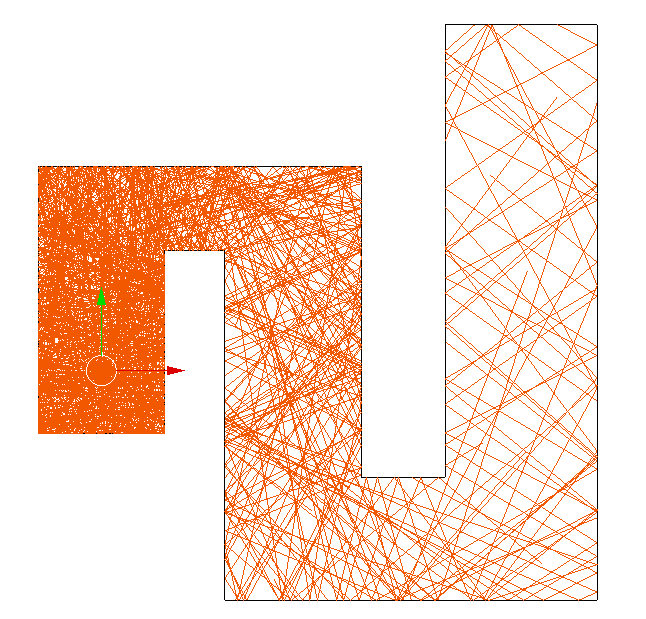
\includegraphics[width=\linewidth]{images/test0}
		\caption{Propagation des rayons dans un labyrinthe}
		\label{test0}
	\end{subfigureth}
	\quad
	\begin{subfigureth}{0.45\textwidth}
		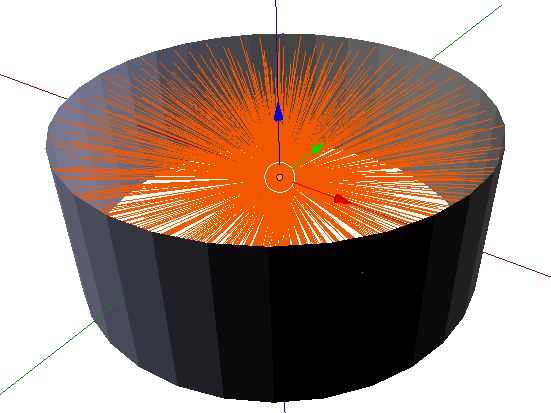
\includegraphics[width=\linewidth]{images/test0bis}
		\caption{Absorption des rayons par une boite englobante autour d'un cylindre ouvert}
		\label{test0bis}
	\end{subfigureth}
\end{figureth}

Nous vérifions aussi que les rayons captés par le récepteur sont bien portés par des cônes. Pour cela nous affichons sur blender uniquement les rayons générant une source image et les traçons depuis celle-ci.

\begin{figureth}
	\begin{subfigureth}{0.45\textwidth}
		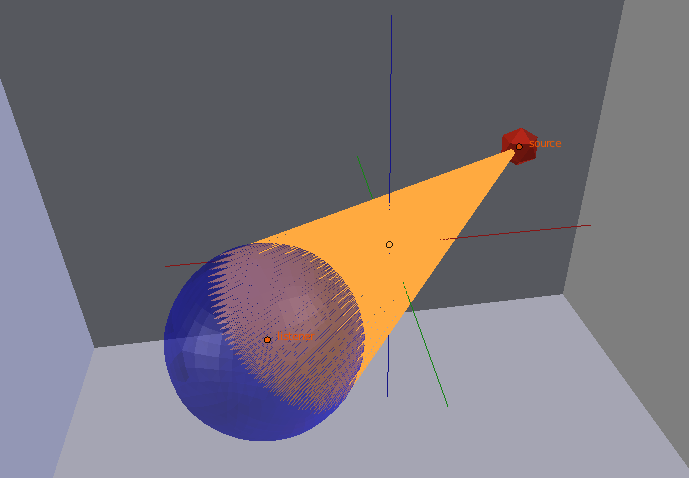
\includegraphics[width=\linewidth]{images/testBeam}
		\caption{Propagation des rayons depuis la source vers le récepteur (100000 rayons au total)}
		\label{testBeam}
	\end{subfigureth}
	\quad
	\begin{subfigureth}{0.45\textwidth}
		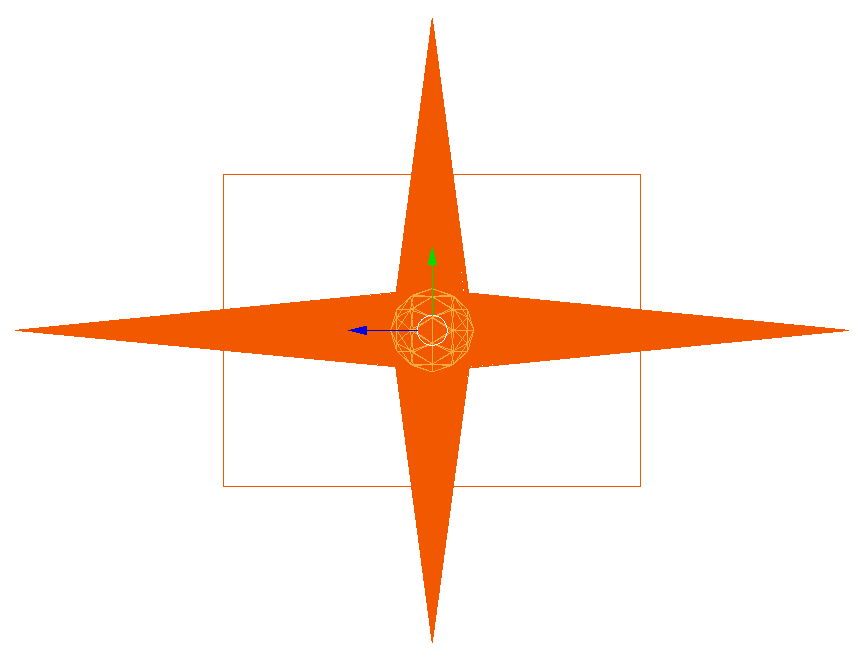
\includegraphics[width=\linewidth]{images/testBeam2}
		\caption{Propagation des rayons depuis les sources-images vers le récepteur à l'ordre 0 et 1  (100000 rayons au total)}
		\label{testBeam2}
	\end{subfigureth}
\end{figureth}



\section{Validation}

\subsection{Décroissance quadratique}
Suite à ces vérifications préliminaires, le premier test à réaliser pour analyser le comportement physique de l'algorithme est celui décrit dans la section \ref{sect_methodecouplee}. Il s'agit de vérifier si l'utilisation d'un grand nombre de rayons et d'un récepteur de diamètre fixe permet de retrouver la loi de décroissance en $d^2$. Pour effectuer ce test, nous plaçons une source et un récepteur de rayons $1m$ au centre d'un cube de $10m$ de coté. Afin de simuler des mesures en espace libre (c'est à dire sans aucune paroi) où le récepteur s'éloigne de la source, nous allons affecter au cube des matériaux $100\%$ absorbants sur toutes ses parois sauf celles sur l'axe des $X$ qui seront $100\%$ réfléchissantes. Ainsi, cela revient à effectuer une mesure tous les $10m$, soit le temps d'aller retour des rayons du centre du cube jusqu'aux parois. N'ayant des réflexions que sur un axe, on reproduit une propagation en espace libre puisque seuls les rayons contenus dans le cône autour de l'axe $X$ conserveront leur énergie. Cependant, les rayons se réfléchissant en X et en -X de manière synchrone, on aura deux fois plus de rayons que si l'on se plaçait en espace libre. Nous pouvons comparer le résultat pour 30 itérations avec la fonction :

\begin{equation*}
f(x) = \frac{2}{x^2}
\end{equation*}

\begin{figureth}
	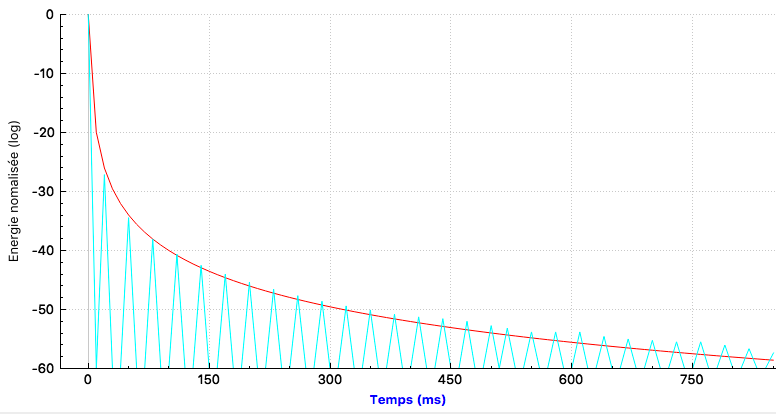
\includegraphics[width=0.8\linewidth]{images/test1}
	\caption{Réponse impulsionnelle en espace libre pour 3 millions de rayons (bleu) échantillonnée à 100Hz et fonction $f(x)=\frac{2}{x^2}$ (rouge)}
	\label{test1}
\end{figureth}

Pour ce test, l'absorption de l'air a été désactivée afin de ne prendre en compte que la décroissance d'énergie portée par les rayons perçus. On observe bien sur la figure \ref{test1} que l'énergie suit la courbe de décroissance quadratique.
 		
		
\subsection{Cas de la salle sphérique}

Le deuxième test consiste à vérifier que l'énergie est bien conservée. Pour cela, nous plaçons une source et un récepteur de diamètre $1m$ au centre d'une sphère $100\%$ réfléchissante de diamètre $4m$. Ainsi à chaque itération, l'ensemble des $1000$ rayons revient se croiser au centre de la sphère et sont donc tous captés par le récepteur. Nous obtenons une réponse impulsionnelle de la forme d'une peigne de Dirac (voir fig. \ref{test2RIR}). L'écart entre chaque pic est de $11,76 ms$ ce qui correspond bien à une distance de $4m$ parcourue à la vitesse du son fixée à $340m/s$. Pour éviter la dispersion des rayons il est nécessaire d'avoir une sphère très bien raffinée. Celle utilisée pour le test possède $320000$ triangles. Par ailleurs, la fréquence d'échantillonnage est descendue à 1000Hz pour s'assurer que les sources-images de chaque itération soient parfaitement synchronisées dans le calcul de l'énergie. On pourra par ailleurs importer les source-images sous Blender et constater qu'elles sont bien réparties sur des sphères dont le diamètre est doublé à chaque itération (voir fig. \ref{test2SI})

\begin{figureth}
	\begin{subfigureth}{0.45\textwidth}
		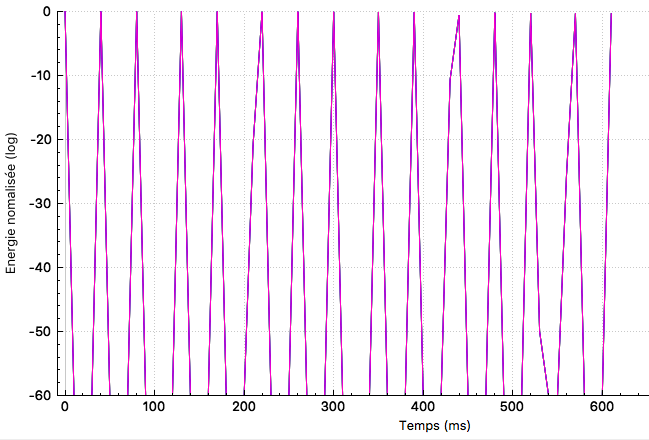
\includegraphics[width=\linewidth]{images/test2RIR}
		\caption{Réponse impulsionnelle dans une sphère 100\% réfléchissante pour 12 itérations}
		\label{test2RIR}
	\end{subfigureth}
	\quad
	\begin{subfigureth}{0.45\textwidth}
		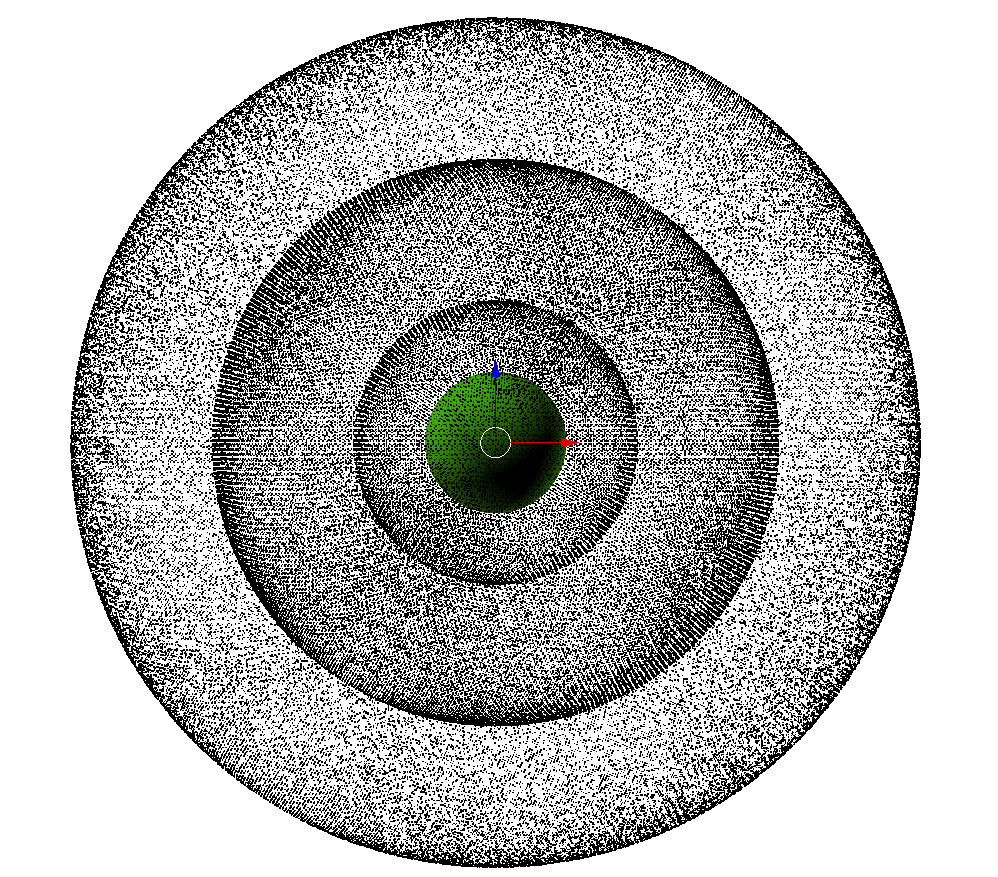
\includegraphics[width=\linewidth]{images/test2SI}
		\caption{Position des sources images dans le cas d'une sphère 100\% réfléchissante pour 4 itérations}
		\label{test2SI}
	\end{subfigureth}
\end{figureth}

Si l'on active l'absorption de l'air, on constate bien que les hautes fréquences sont plus absorbées que les basses fréquences en fonction de la distance (voir fig. \ref{test2absair}). Notamment au bout de 1700ms soit 578m, les fréquences à 8kHz ont quasiment totalement été absorbées par l'air, pour une température de 20°C et une pression relative de 50\%.

%On peut aussi vérifier ce comportement dans le cas plus général d'un ellipsoïde de révolution. Celui-ci peut être créé sous Blender à l'aide de l'add-on "\textit{Extra Objects}" en configurant un objet de type "\textit{XYZ Math Surface}". Nous créons alors un ellipsoïde avec les équations suivantes :

\begin{figureth}
	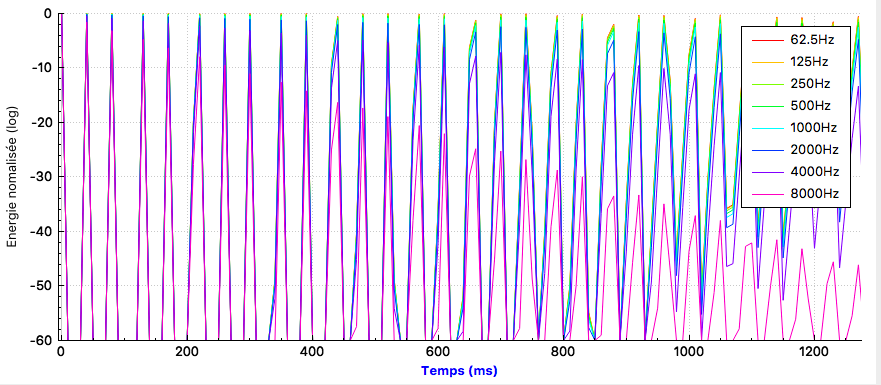
\includegraphics[width=\linewidth]{images/test2absair}
	\caption{Réponse impulsionnelle dans une sphère de $20m$ de diamètre, 100\% réfléchissante, pour 30 itérations avec absorption de l'air}
	\label{test2absair}
\end{figureth}

\subsection{Cas de la salle cubique}

Le dernier test consiste à comparer les résultats de calcul avec une formule analytique pour une pièce de type pavé droit. La formule \cite[p. 182-189]{mcgovern} est la suivante : 

\begin{align}
A &=  (-1)^i \\
B &= i + 0,5 - 0,5 \times (-1)^i \\
P_{si} &= A \times P_s + B \times D
\end{align}

Que l'on peut plus simplement écrire :

\begin{align}
P_{si} = i \times D + P_s \times (-1)^i
\end{align}

Avec : \\
$i \in (-n, n)$ et $n \in \mathbb{N}$ \\
$P_{si}$ : La coordonnée de la position de la source image selon X, Y ou Z \\
$P_s$ : La coordonnée de la position de la source selon X, Y ou Z \\
$D$ : La dimension de la salle selon X, Y ou Z \\

On constate alors qu'on a une superposition des sources-images dans l'espace. Cette précision se dégrade légèrement lorsque le nombre de rayons ou le nombre d'itérations augmente à cause de l'imprécision machine; elle reste cependant acceptable. Nous calculons l'erreur relative de la distance au récepteur pour les sources-images expérimentales obtenues par lancer de rayons et les sources-images théoriques obtenues par formule analytique.
\begin{align}
\epsilon_{rel} = \frac{D_{exp}-D_{theo}}{D_{theo}}
\end{align}

La précision est de l'ordre du centième de pour-cent et augmente légèrement lorsqu'on s'éloigne du récepteur (voir fig. \ref{test3}).
En terme de mesure d'énergie, on assigne à chaque source-image une énergie de $\frac{1}{d^2}$ où $d$ est sa distance par rapport au récepteur. Nous traçons de la même manière l'erreur relative sur les énergies.


On constate que celle-ci à une valeur moyenne de $0,6\%$ est qu'elle reste toujours inférieure à 1\% jusqu'à un certain seuil (voir fig. \ref{test3bis}).

\begin{figureth}
	\begin{subfigureth}{0.8\textwidth}
		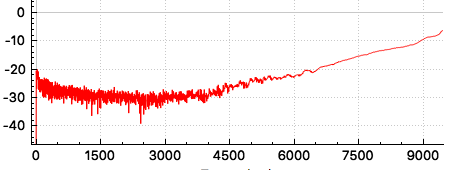
\includegraphics[width=\linewidth]{images/test3}
		\caption{Erreur relative des distances (\% en échelle log) pour une salle cubique de 10m de coté, 1000000 rayons et 20 itérations}
		\label{test3}
	\end{subfigureth}
	%\quad
	\begin{subfigureth}{0.8\textwidth}
		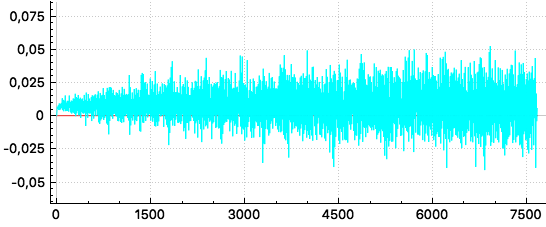
\includegraphics[width=\linewidth]{images/test3bis}
		\caption{Erreur relative des énergies (\%) pour une salle cubique de 10m de coté, 100000 rayons et 10 itérations}
		\label{test3bis}
	\end{subfigureth}
\end{figureth}
		
		

\section{Interface utilisateur} \label{sect_add-on}

La force de ce développement logiciel est que l'utilisateur n'a pas besoin d'effectuer de manipulations complexes pour obtenir les résultats de calcul d'acoustique de salle. Il pourra travailler directement sur son maillage dans le logiciel \gls{cao} et lancer le calcul. Blender permet de développer des scripts en Python qui peuvent par la suite être installés sous forme de \textit{add-on}. L'interface homme-machine de Blender est donc complètement modulable et personnalisable. Le add-on développé dans la cadre de ce projet possède quelques boutons. En utilisant le bouton "Run", Blender transforme les faces des objets sélectionnés en triangle et les exporte au format \gls{obj} (dans le répertoire où se trouve l'exécutable créé en C++). Dans le fichier de maillage, chaque objet est différencié par un en-tête comprenant son nom. S'en suit les coordonnées de l'ensemble de ses sommets (ou vertices), de ses textures et de ses normales. Ensuite sont regroupées par matériaux, les faces par combinaison de trois vertices, d'une texture et d'une normale. Un vecteur de sommets et un vecteur de normales sont remplis face par face en conservant le même ordre. Ces deux vecteurs stockent ainsi la totalité du maillage. Les textures quant à elles ne nous sont pas utiles. Les coefficients d'absorption des matériaux sont aussi assemblés dans un vecteur en les classant face par face en respectant l'ordre établi précédemment.

Par défaut, une source et un récepteur sont positionnés au point [0, 0, 0]. Le rayon de mesure du récepteur est de 1m. Cependant, l'utilisateur pourra changer ces paramètres en créant des objets source et récepteur dans Blender. Pour être reconnus et discriminés du maillage, ces objets doivent respectivement comporter les mots "\textit{source}" et "\textit{listener}" dans leur nom. L'algorithme déterminera alors le centre des objets sources et des récepteurs en calculant la moyenne des coordonnées des sommets. Le rayon de mesure du récepteur correspond au rayon de la sphère circonscrite à l'objet "\textit{listener}". Notons qu'il est possible de placer plusieurs sources. L'ensemble des calculs se réaliseront séquentiellement pour une source après l'autre. Un seul récepteur est pris en compte. L'add-on Blender permet de mettre à jour uniquement les informations sur les sources et récepteurs sans avoir besoin de recharger tout le maillage.
Par ailleurs l'utilisateur assignera aux différentes parois un type de matériau en faisant apparaitre dans son nom la référence du matériau issue de la base de donnée Odéon (voir section \ref{sect_lectMat}). 


\begin{figureth}
	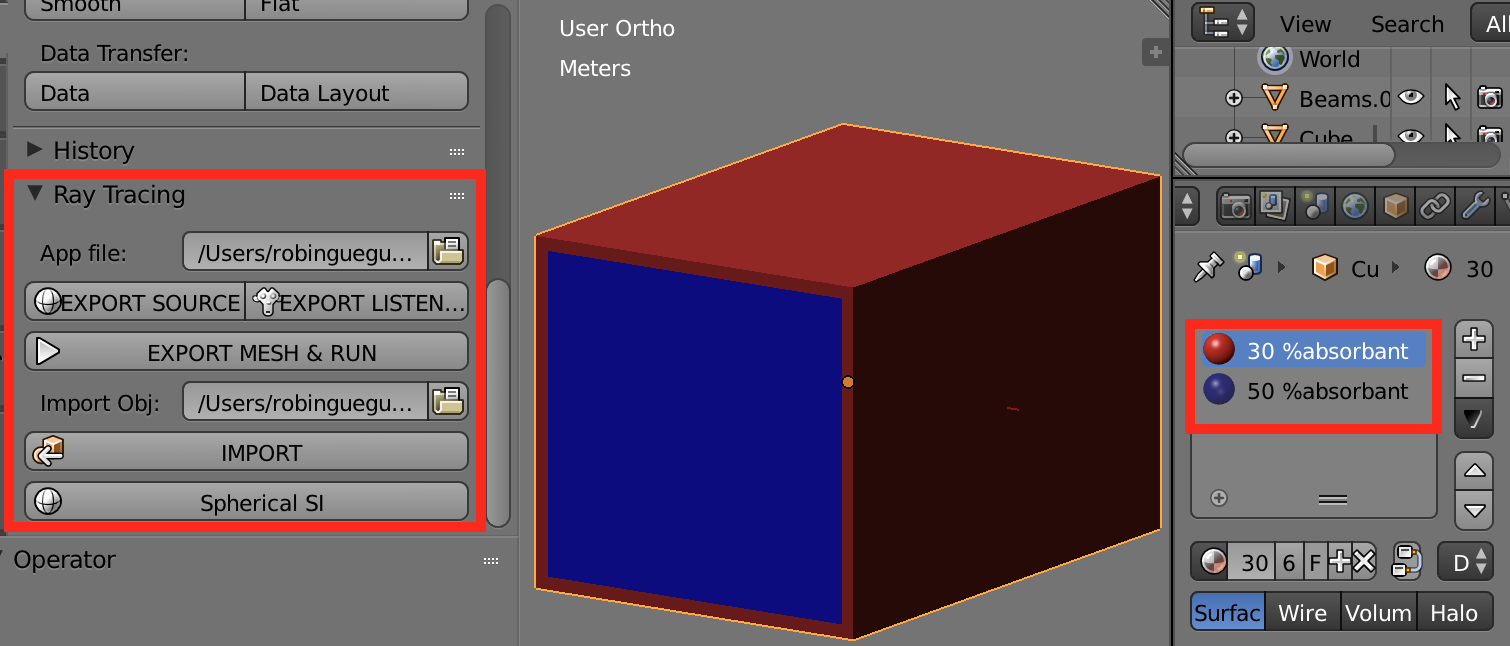
\includegraphics[width=\linewidth]{images/add-on}
	\caption{Add-on Blender et assignation des matériaux}
\end{figureth}

\section{Traitement du signal} \label{sect_TDS}

L'analyse de résultats d'une étude acoustique peut parfois être délicate et difficile pour les personnes extérieurs au milieu. Le résultat final qui pourra être analysé par le plus grand nombre est le signal audio de sortie. Même si l'analyse d'un signal audio nécessite une grande finesse auditive, elle présente pour avantage d'être accessible par une simple écoute. Pour obtenir le son réverbéré, il s'agit de convoluer le signal d'origine avec les \gls{fir}. Un \gls{fir} est une \gls{rir} exprimé en pression tel que :

\begin{equation}
P = \sqrt{E}
\end{equation}

Avec : \\
$P$ : La pression sonore normalisée \\
$E$ : L'énergie normalisée \\

Convoluer ces signaux revient à multiplier point par point le fichier audio avec les \gls{fir} dans le domaine de Fourier (fréquenciel).
On utilise pour cela des fichiers au format \gls{wav}. Dans le cas de longs signaux, il est judicieux d'utiliser une convolution partitionnée afin de réduire le stockage de données et accélérer les calculs \cite[2. Algorithm overview ]{partition}. 

L'algorithme mis en place fonctionne de la manière suivante (voir fig. \ref{DiagTdS}) :
\begin{figureth}
	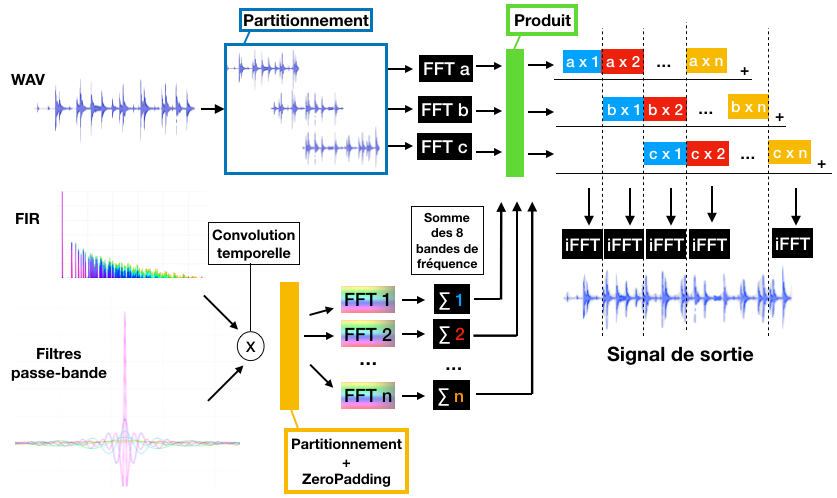
\includegraphics[width=\linewidth]{images/DiagTdS}
	\caption{Schéma du processus de convolution partitionnée}
	\label{DiagTdS}
\end{figureth}

Premièrement, on fixe la longueur des partitions à $n$ échantillons tel que $n$ soit une puissance de 2 (typiquement 1024). Dans un premier temps, le signal audio est découpé par tranches de $n$ échantillons et chaque tranche recouvre la précédente sur la moitié de sa taille. Chacune d'entre elles est ensuite passées dans le domaine spectral par \gls{fft}. Dans un second temps les \gls{fir} sont convolués temporellement à des filtres passe-bande (voir fig. \ref{filtres}), c'est à dire que chaque pic des \gls{fir} sera multiplié par le filtre passe-bande de la fréquence correspondante. Les huit signaux de sortie sont alors découpé par tranches de $n/2$ échantillons que l'on fait précéder de $n/2$ zéros. Ce procédé se nomme "\textit{ZeroPadding}" et permet d'éviter les effets de crénelage (\textit{aliasing}) lors de la convolution de deux signaux. En effet, les spectres des signaux présentent sur leur partie négative un repliement qui apporte de l'information redondante lors de la convolution. C'est pour cette même raison que les partitions du signal audio ont un recouvrement de $n/2$ échantillons. Ainsi, seuls les $n/2$ derniers échantillons du résultat de convolution sont utiles. Avant de pouvoir effectuer cette opération il faut passer les filtres dans le domaine spectral et sommer les huit bandes de fréquence. Une par une les partitions du signal audio sont convoluées aux filtres et à chaque nouvelle partition, on décale le résultat de $n/2$ échantillons. On pourra alors sommer les résultats et effectuer une transformée de Fourier inverse pour récupérer le signal de sortie. Celui-ci sera identique au signal d'entrée à la différence qu'il sera réverbéré, c'est à dire que chaque pic de la \gls{rir} répétera le signal d'entrée en écho.

\begin{figureth}
	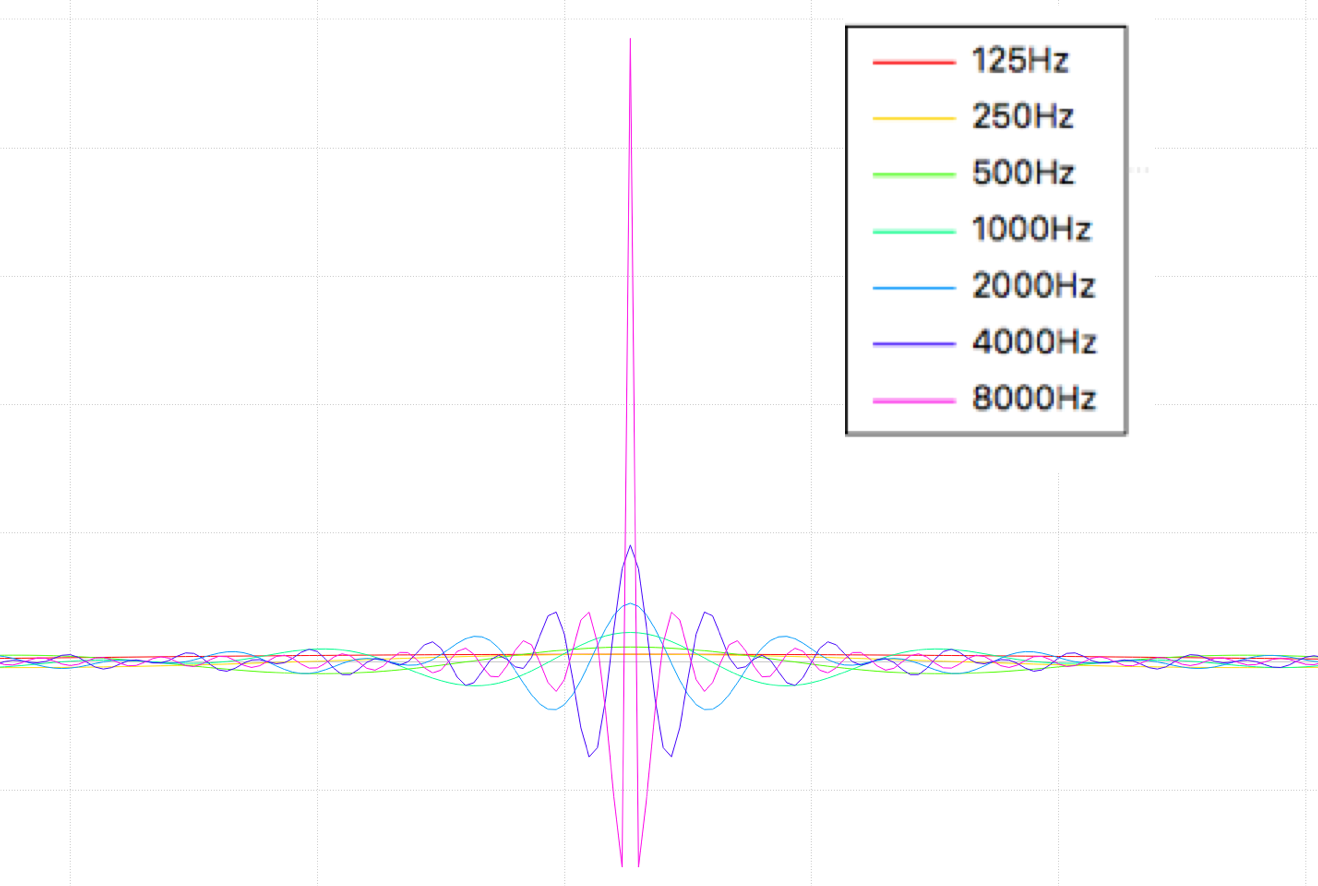
\includegraphics[width=0.9\linewidth]{images/filtres}
	\caption{Filtres fréquenciels passe-bande}
	\label{filtres}
\end{figureth}




	
\chapter*{Conclusion}
\addcontentsline{toc}{chapter}{Conclusion}

Dans cette partie, nous avons présenté les problématiques soulevées par une étude acoustique d'un monument antique. La géométrie complexe de ce type de bâtiment et leur taille colossale impose l'utilisation de méthodes de calcul approchées. Ainsi, par simulation des réflexions et absorptions des parois, il est possible d'étudier la réverbération d'une salle. Malgré les approximations inéluctables du modèle, nous avons prouvé que les lois de la physique sont respectées. Un algorithme rapide a été mis en place pour permettre aux utilisateurs de tester facilement et rapidement leurs hypothèses architecturales. Ainsi, le temps de calcul devient peu sensible aux nombres d'éléments du maillage ce qui est souvent limitant dans ce genre d'étude. L'implémentation d'une \gls{ihm} sous Blender s'interface dans la continuité de l'étude présentée dans la partie \ref{part_1} de ce document. 

La figure \ref{synopsis} présente de manière synthétique l'architecture logicielle développée au cours du projet. 
\begin{figureth}
	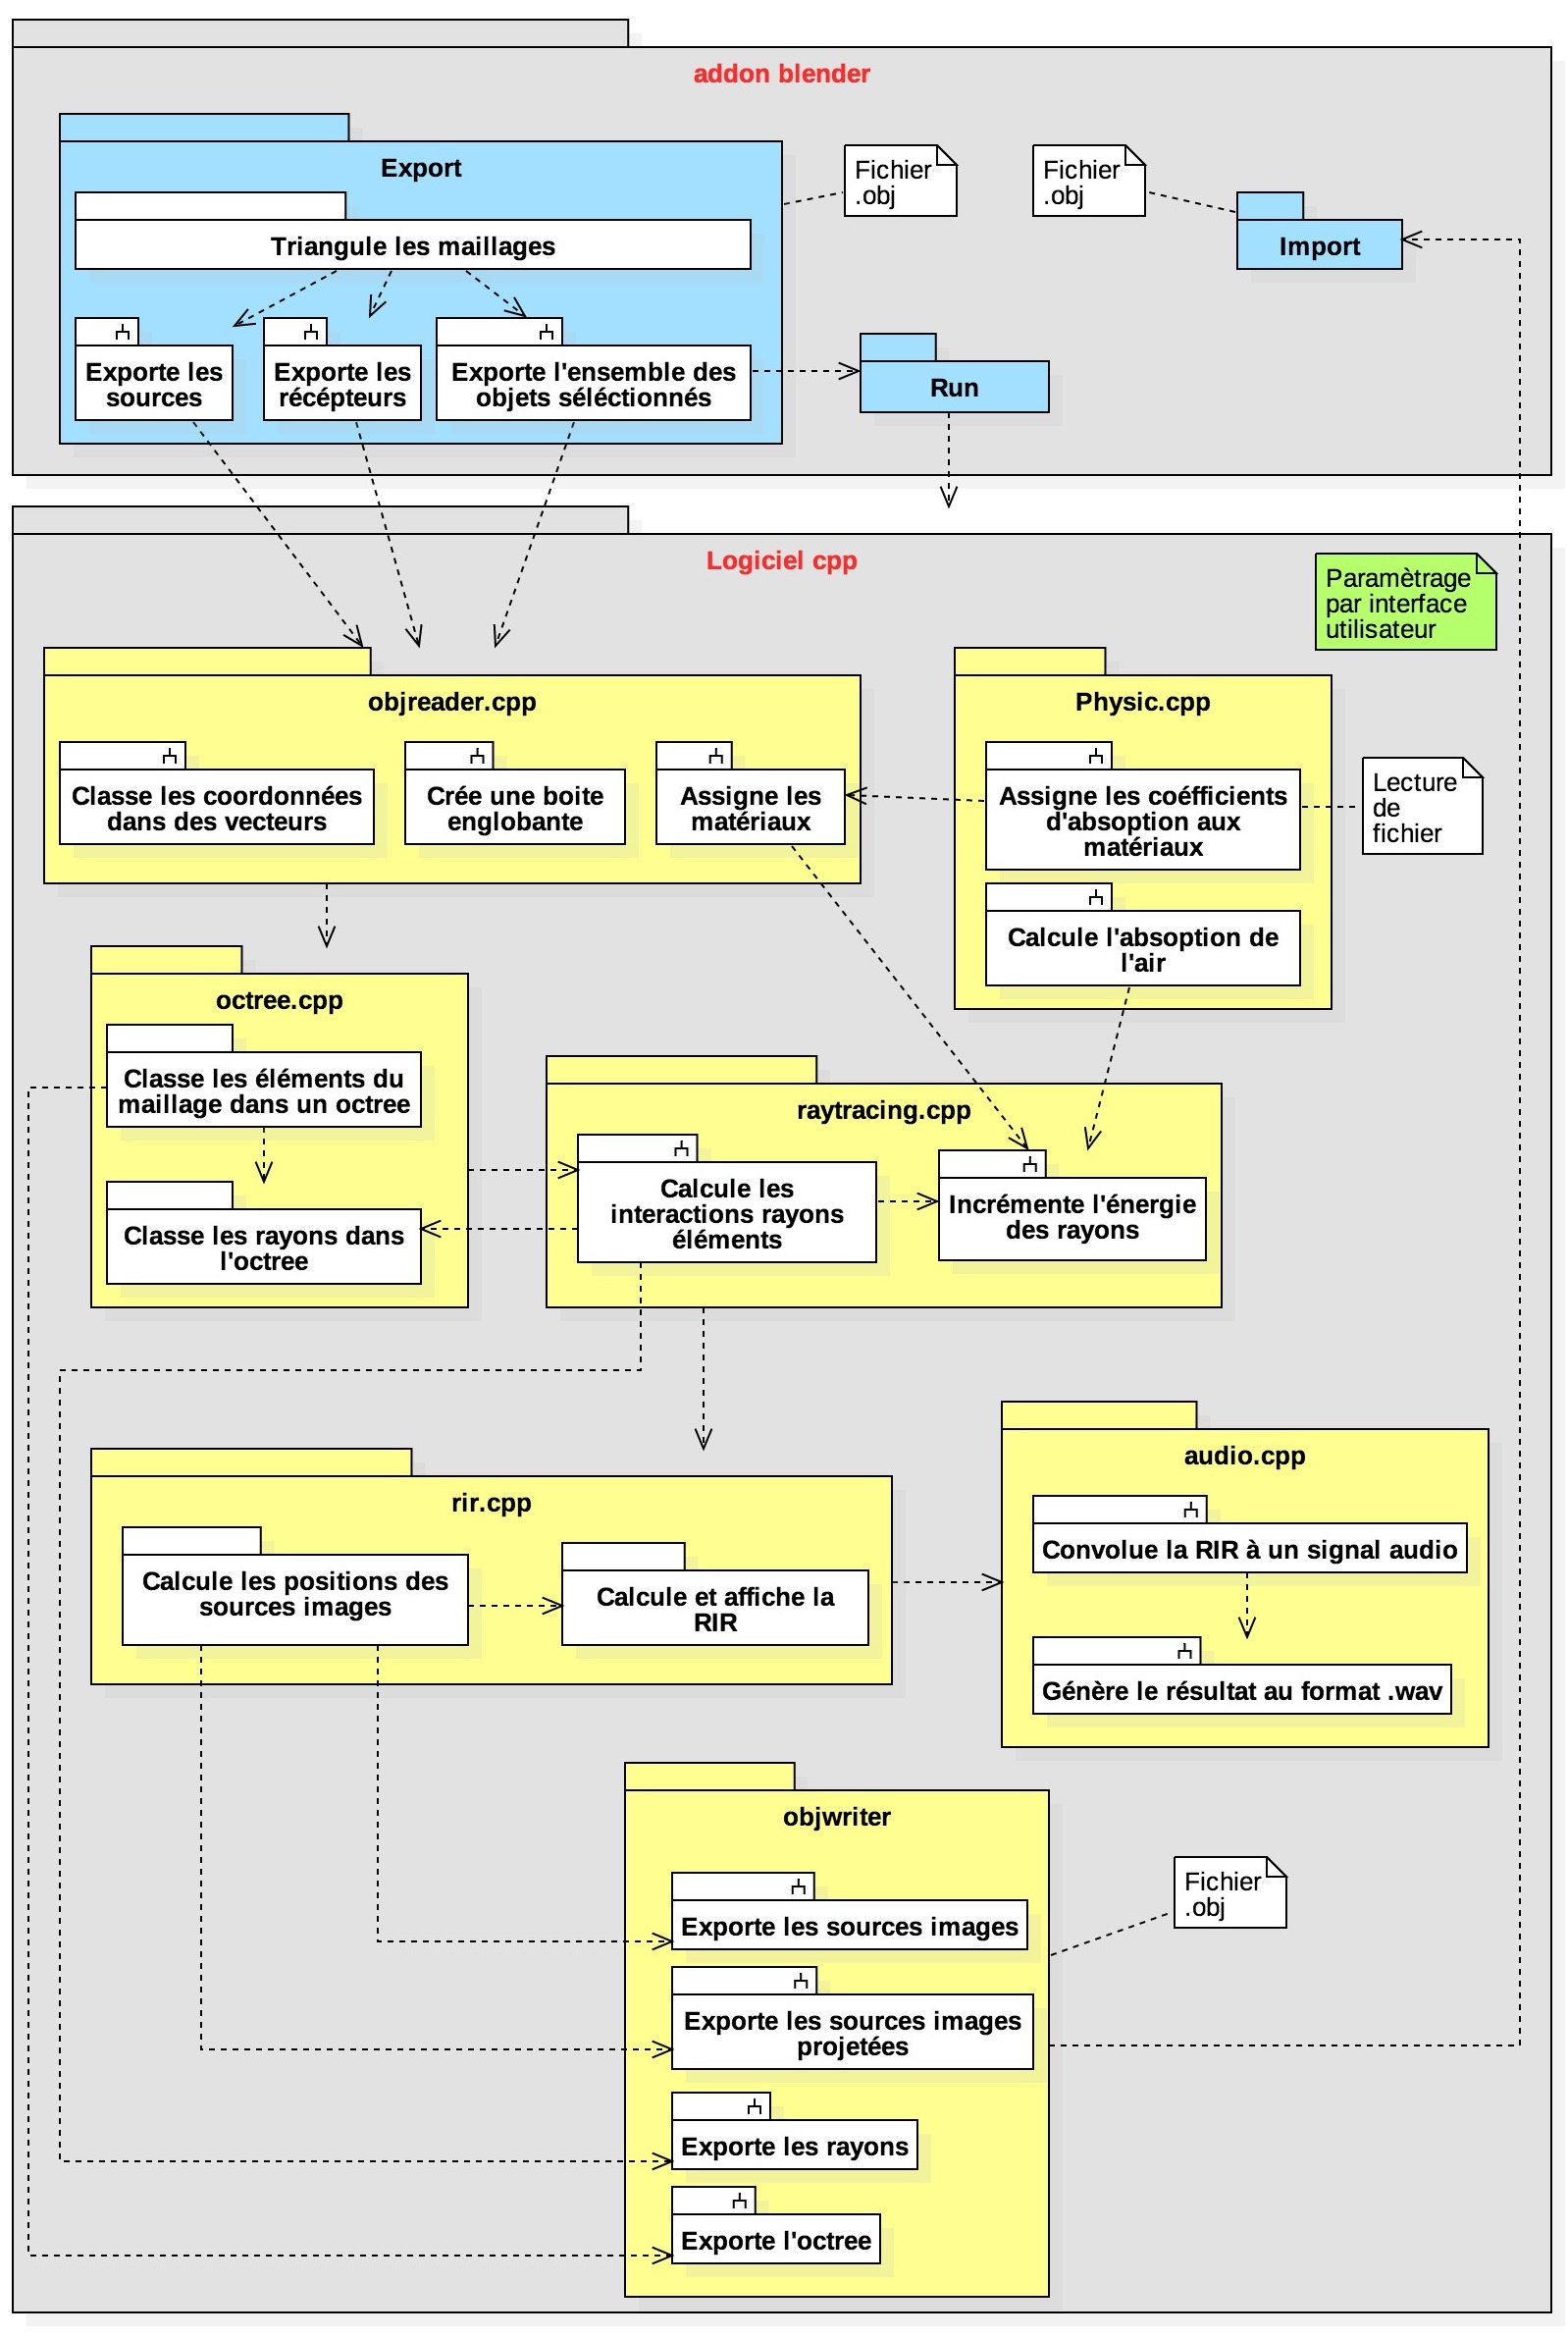
\includegraphics[width=\linewidth]{images/synopsis}
	\caption{Synopsis de l'architecture logiciel développé pour le calcul d'acoustique de salle}
	\label{synopsis}
\end{figureth}

Le fonctionnement de l'algorithme développé a été présenté en détail de même que les différents outils d'analyse qui en découlent. Il est alors possible d'étudier le graphe temporel de réverbération du bâtiment ainsi que la position dans l'espace des différentes réflexions sonores. Ces résultats pourront aussi être analysés à l'oreille en écoutant le son réverbéré émis depuis une ou plusieurs sources et entendu par un auditeur virtuel placé dans le bâtiment.

De nombreuses possibilités d'améliorations restent à l'étude comme par exemple l'écoute en temps réel. Il serait par exemple possible d'écouter les signaux réverbérés en 3D grâce à des filtres binauraux. Ceux-ci modifient le signal perçu par chacune des deux oreilles afin de donner l'illusion d'espace et de profondeur. Tout en restant en position statique, l'auditeur pourra orienter son regard selon différentes directions et écouter en temps réel le son changer. Cette option fonctionne sous Matlab avec un contrôle de la direction au clavier ou à l'aide d'un casque avec "\textit{Head Tracker"}. Ce type de casque possède un gyroscope qui actualise la direction du regard en temps réel et permet d'augmenter considérable la sensation immersive. Par ailleurs, ce code, que ce soit sous Matlab ou en C++ (avec add-on Blender), est distribué en open-source. 

Il y a par ailleurs de nombreuses améliorations envisageables au niveau graphique. Comment visualiser des résultats de calculs acoustiques ? Quelles sont les informations indispensables à recueillir pour un archéologue voulant étudier l'acoustique d'un monument ? Voici des questions qui se posent à l'issue de ce développement.

De la même manière, est-il essentiel d'ajouter les effets de diffraction au modèle ? Si oui, quelle est la meilleur méthode ? Pourrait-on traiter de manière locale certains comportements acoustiques et les insérer ensuite dans le modèle par lancer de rayons ? Typiquement, pourrait-on analyser par méthode de résolution exacte (voir section \ref{sect_resExacte}) le comportement acoustique d'une colonne, ou de tout autre ornement avec un fort niveau de détail, puis de l'incorporer de manière analytique dans l'outil de lancer de rayons ? 

Nous l'avons déjà évoqué dans la section \ref{sect_rayon}, mais il serait également interessant d'utiliser des sources dont la directivité n'est pas uniforme. Cela serait d'ailleurs plus représentatif des cas réels et notamment de l'usage fait à Orange à l'origine du théâtre. Les sons étaient alors émis par des instruments de musique ou par la voix humaine éventuellement amplifiée par un masque.

Ce sont des questions que nous allons pouvoir approfondir dans le partie suivante. Celle-ci se propose d'explorer toutes les possibilités de ce nouvel outil de calcul acoustique appliqué à notre objet d'étude : le théâtre d'Orange. Nous tenterons d'analyser des hypothèses archéologiques précises grâce à l'étude acoustique du bâtiment.



\newpage
	
% Biblio
 \bibliographystyle{francaissc}
 \bibliography{Part2/Biblio}
\addcontentsline{toc}{chapter}{Références}
